\documentclass[twoside]{book}

% Packages required by doxygen
\usepackage{fixltx2e}
\usepackage{calc}
\usepackage{doxygen}
\usepackage[export]{adjustbox} % also loads graphicx
\usepackage{graphicx}
\usepackage[utf8]{inputenc}
\usepackage{makeidx}
\usepackage{multicol}
\usepackage{multirow}
\PassOptionsToPackage{warn}{textcomp}
\usepackage{textcomp}
\usepackage[nointegrals]{wasysym}
\usepackage[table]{xcolor}

% Font selection
\usepackage[T1]{fontenc}
\usepackage[scaled=.90]{helvet}
\usepackage{courier}
\usepackage{amssymb}
\usepackage{sectsty}
\renewcommand{\familydefault}{\sfdefault}
\allsectionsfont{%
  \fontseries{bc}\selectfont%
  \color{darkgray}%
}
\renewcommand{\DoxyLabelFont}{%
  \fontseries{bc}\selectfont%
  \color{darkgray}%
}
\newcommand{\+}{\discretionary{\mbox{\scriptsize$\hookleftarrow$}}{}{}}

% Page & text layout
\usepackage{geometry}
\geometry{%
  a4paper,%
  top=2.5cm,%
  bottom=2.5cm,%
  left=2.5cm,%
  right=2.5cm%
}
\tolerance=750
\hfuzz=15pt
\hbadness=750
\setlength{\emergencystretch}{15pt}
\setlength{\parindent}{0cm}
\setlength{\parskip}{3ex plus 2ex minus 2ex}
\makeatletter
\renewcommand{\paragraph}{%
  \@startsection{paragraph}{4}{0ex}{-1.0ex}{1.0ex}{%
    \normalfont\normalsize\bfseries\SS@parafont%
  }%
}
\renewcommand{\subparagraph}{%
  \@startsection{subparagraph}{5}{0ex}{-1.0ex}{1.0ex}{%
    \normalfont\normalsize\bfseries\SS@subparafont%
  }%
}
\makeatother

% Headers & footers
\usepackage{fancyhdr}
\pagestyle{fancyplain}
\fancyhead[LE]{\fancyplain{}{\bfseries\thepage}}
\fancyhead[CE]{\fancyplain{}{}}
\fancyhead[RE]{\fancyplain{}{\bfseries\leftmark}}
\fancyhead[LO]{\fancyplain{}{\bfseries\rightmark}}
\fancyhead[CO]{\fancyplain{}{}}
\fancyhead[RO]{\fancyplain{}{\bfseries\thepage}}
\fancyfoot[LE]{\fancyplain{}{}}
\fancyfoot[CE]{\fancyplain{}{}}
\fancyfoot[RE]{\fancyplain{}{\bfseries\scriptsize Generated by Doxygen }}
\fancyfoot[LO]{\fancyplain{}{\bfseries\scriptsize Generated by Doxygen }}
\fancyfoot[CO]{\fancyplain{}{}}
\fancyfoot[RO]{\fancyplain{}{}}
\renewcommand{\footrulewidth}{0.4pt}
\renewcommand{\chaptermark}[1]{%
  \markboth{#1}{}%
}
\renewcommand{\sectionmark}[1]{%
  \markright{\thesection\ #1}%
}

% Indices & bibliography
\usepackage{natbib}
\usepackage[titles]{tocloft}
\setcounter{tocdepth}{3}
\setcounter{secnumdepth}{5}
\makeindex

% Hyperlinks (required, but should be loaded last)
\usepackage{ifpdf}
\ifpdf
  \usepackage[pdftex,pagebackref=true]{hyperref}
\else
  \usepackage[ps2pdf,pagebackref=true]{hyperref}
\fi
\hypersetup{%
  colorlinks=true,%
  linkcolor=blue,%
  citecolor=blue,%
  unicode%
}

% Custom commands
\newcommand{\clearemptydoublepage}{%
  \newpage{\pagestyle{empty}\cleardoublepage}%
}

\usepackage{caption}
\captionsetup{labelsep=space,justification=centering,font={bf},singlelinecheck=off,skip=4pt,position=top}

%===== C O N T E N T S =====

\begin{document}

% Titlepage & ToC
\hypersetup{pageanchor=false,
             bookmarksnumbered=true,
             pdfencoding=unicode
            }
\pagenumbering{alph}
\begin{titlepage}
\vspace*{7cm}
\begin{center}%
{\Large Sprite\+Walker }\\
\vspace*{1cm}
{\large Generated by Doxygen 1.8.13}\\
\end{center}
\end{titlepage}
\clearemptydoublepage
\pagenumbering{roman}
\tableofcontents
\clearemptydoublepage
\pagenumbering{arabic}
\hypersetup{pageanchor=true}

%--- Begin generated contents ---
\chapter{Hierarchical Index}
\section{Class Hierarchy}
This inheritance list is sorted roughly, but not completely, alphabetically\+:\begin{DoxyCompactList}
\item \contentsline{section}{Actor\+Assets}{\pageref{class_actor_assets}}{}
\item \contentsline{section}{Asset\+Manager}{\pageref{class_asset_manager}}{}
\item \contentsline{section}{C\+Rule\+Set}{\pageref{class_c_rule_set}}{}
\begin{DoxyCompactList}
\item \contentsline{section}{Hero\+Rules}{\pageref{class_hero_rules}}{}
\item \contentsline{section}{Monster\+Rules}{\pageref{class_monster_rules}}{}
\item \contentsline{section}{Scheusal\+Rules}{\pageref{class_scheusal_rules}}{}
\item \contentsline{section}{Villager\+Rules}{\pageref{class_villager_rules}}{}
\end{DoxyCompactList}
\item \contentsline{section}{C\+Utilities}{\pageref{class_c_utilities}}{}
\item \contentsline{section}{mfg\+:\+:Engine}{\pageref{classmfg_1_1_engine}}{}
\item \contentsline{section}{Line\+Edit\+Widget}{\pageref{class_line_edit_widget}}{}
\item Q\+Action\begin{DoxyCompactList}
\item \contentsline{section}{C\+Menu\+Action}{\pageref{class_c_menu_action}}{}
\end{DoxyCompactList}
\item Q\+Dialog\begin{DoxyCompactList}
\item \contentsline{section}{C\+Actor\+Dialog}{\pageref{class_c_actor_dialog}}{}
\end{DoxyCompactList}
\item Q\+Graphics\+Item\begin{DoxyCompactList}
\item \contentsline{section}{Sprite}{\pageref{class_sprite}}{}
\begin{DoxyCompactList}
\item \contentsline{section}{Actor}{\pageref{class_actor}}{}
\end{DoxyCompactList}
\end{DoxyCompactList}
\item Q\+Graphics\+Scene\begin{DoxyCompactList}
\item \contentsline{section}{C\+Tile\+Scene}{\pageref{class_c_tile_scene}}{}
\end{DoxyCompactList}
\item Q\+Graphics\+View\begin{DoxyCompactList}
\item \contentsline{section}{C\+Game\+View}{\pageref{class_c_game_view}}{}
\end{DoxyCompactList}
\item Q\+Main\+Window\begin{DoxyCompactList}
\item \contentsline{section}{Main\+Window}{\pageref{class_main_window}}{}
\end{DoxyCompactList}
\item Q\+Object\begin{DoxyCompactList}
\item \contentsline{section}{C\+Key\+Press\+Consumer}{\pageref{class_c_key_press_consumer}}{}
\item \contentsline{section}{Sequential\+G\+U\+ID}{\pageref{class_sequential_g_u_i_d}}{}
\item \contentsline{section}{Sprite}{\pageref{class_sprite}}{}
\end{DoxyCompactList}
\item Q\+Thread\begin{DoxyCompactList}
\item \contentsline{section}{Collision\+Thread}{\pageref{class_collision_thread}}{}
\end{DoxyCompactList}
\item Q\+Widget\begin{DoxyCompactList}
\item \contentsline{section}{Console\+Widget}{\pageref{class_console_widget}}{}
\end{DoxyCompactList}
\item \contentsline{section}{Scene\+Manager}{\pageref{class_scene_manager}}{}
\item \contentsline{section}{mfg\+:\+:Stats}{\pageref{structmfg_1_1_stats}}{}
\end{DoxyCompactList}

\chapter{Class Index}
\section{Class List}
Here are the classes, structs, unions and interfaces with brief descriptions\+:\begin{DoxyCompactList}
\item\contentsline{section}{\hyperlink{class_actor}{Actor} \\*
\begin{DoxyItemize}
\item provides a specific type of \hyperlink{class_sprite}{Sprite} that defines both non player and player characters  
\end{DoxyItemize}}{\pageref{class_actor}}{}
\item\contentsline{section}{\hyperlink{class_actor_dialog}{Actor\+Dialog} \\*
\begin{DoxyItemize}
\item defines a dialog box for actor properties 
\end{DoxyItemize}}{\pageref{class_actor_dialog}}{}
\item\contentsline{section}{\hyperlink{class_asset_manager}{Asset\+Manager} \\*
\begin{DoxyItemize}
\item defines a manager for \hyperlink{class_sprite}{Sprite} assets 
\end{DoxyItemize}}{\pageref{class_asset_manager}}{}
\item\contentsline{section}{\hyperlink{class_console_widget}{Console\+Widget} \\*
\begin{DoxyItemize}
\item Provides a console for use in a \hyperlink{class_game_scene}{Game\+Scene} 
\end{DoxyItemize}}{\pageref{class_console_widget}}{}
\item\contentsline{section}{\hyperlink{classmfg_1_1_engine}{mfg\+::\+Engine} \\*
\begin{DoxyItemize}
\item a game engine 
\end{DoxyItemize}}{\pageref{classmfg_1_1_engine}}{}
\item\contentsline{section}{\hyperlink{class_game_scene}{Game\+Scene} \\*
\begin{DoxyItemize}
\item creates a graphic scene used for game play 
\end{DoxyItemize}}{\pageref{class_game_scene}}{}
\item\contentsline{section}{\hyperlink{class_hero_rules}{Hero\+Rules} \\*
\begin{DoxyItemize}
\item define rules for a Hero \hyperlink{class_actor}{Actor} 
\end{DoxyItemize}}{\pageref{class_hero_rules}}{}
\item\contentsline{section}{\hyperlink{class_key_press_consumer}{Key\+Press\+Consumer} \\*
\begin{DoxyItemize}
\item traps keyboard events so arrow keys can be filtered from application 
\end{DoxyItemize}}{\pageref{class_key_press_consumer}}{}
\item\contentsline{section}{\hyperlink{class_main_window}{Main\+Window} \\*
\begin{DoxyItemize}
\item Defines Main window for application 
\end{DoxyItemize}}{\pageref{class_main_window}}{}
\item\contentsline{section}{\hyperlink{class_monster_rules}{Monster\+Rules} \\*
\begin{DoxyItemize}
\item Rule set for a Monster 
\end{DoxyItemize}}{\pageref{class_monster_rules}}{}
\item\contentsline{section}{\hyperlink{class_rule_set}{Rule\+Set} \\*
\begin{DoxyItemize}
\item define rules for characters 
\end{DoxyItemize}}{\pageref{class_rule_set}}{}
\item\contentsline{section}{\hyperlink{class_scene_manager}{Scene\+Manager} \\*
\begin{DoxyItemize}
\item defines a \hyperlink{class_scene_manager}{Scene\+Manager} 
\end{DoxyItemize}}{\pageref{class_scene_manager}}{}
\item\contentsline{section}{\hyperlink{class_scheusal_rules}{Scheusal\+Rules} \\*
\begin{DoxyItemize}
\item Rule set for a Scheusal (Zombie) 
\end{DoxyItemize}}{\pageref{class_scheusal_rules}}{}
\item\contentsline{section}{\hyperlink{class_sequential_g_u_i_d}{Sequential\+G\+U\+ID} \\*
\begin{DoxyItemize}
\item define a class for creating a Sequential G\+U\+ID 
\end{DoxyItemize}}{\pageref{class_sequential_g_u_i_d}}{}
\item\contentsline{section}{\hyperlink{class_sprite}{Sprite} \\*
\begin{DoxyItemize}
\item defines a \hyperlink{class_sprite}{Sprite} 
\end{DoxyItemize}}{\pageref{class_sprite}}{}
\item\contentsline{section}{\hyperlink{structmfg_1_1_stats}{mfg\+::\+Stats} \\*The \hyperlink{structmfg_1_1_stats}{Stats} struct -\/ defines the stats for a character }{\pageref{structmfg_1_1_stats}}{}
\item\contentsline{section}{\hyperlink{class_utilities}{Utilities} \\*
\begin{DoxyItemize}
\item defines a \hyperlink{class_utilities}{Utilities} class for functions required, mostly static functions 
\end{DoxyItemize}}{\pageref{class_utilities}}{}
\item\contentsline{section}{\hyperlink{class_villager_rules}{Villager\+Rules} \\*
\begin{DoxyItemize}
\item Rule set for a Villager 
\end{DoxyItemize}}{\pageref{class_villager_rules}}{}
\end{DoxyCompactList}

\chapter{Class Documentation}
\hypertarget{class_actor}{}\section{Actor Class Reference}
\label{class_actor}\index{Actor@{Actor}}


The \hyperlink{class_actor}{Actor} class -- provides a specific type of \hyperlink{class_sprite}{Sprite} that defines both non player and player characters .  




{\ttfamily \#include $<$actor.\+h$>$}

Inheritance diagram for Actor\+:\begin{figure}[H]
\begin{center}
\leavevmode
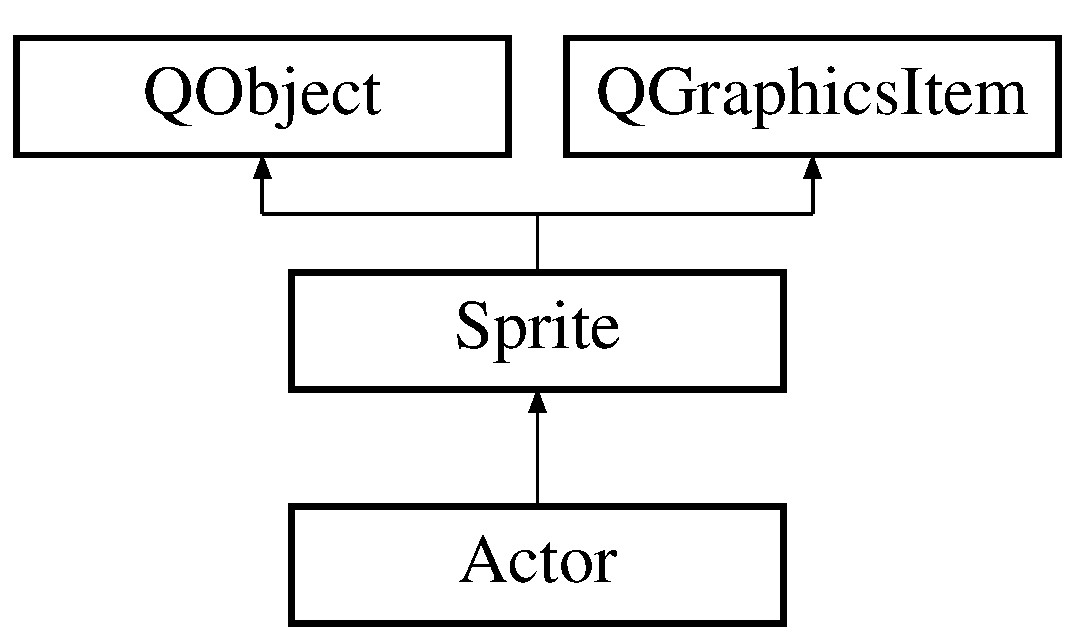
\includegraphics[height=3.000000cm]{class_actor}
\end{center}
\end{figure}
\subsection*{Public Slots}
\begin{DoxyCompactItemize}
\item 
\mbox{\Hypertarget{class_actor_abfb178899dad2f9e42f16280c7fe31e6}\label{class_actor_abfb178899dad2f9e42f16280c7fe31e6}} 
virtual void {\bfseries mouse\+Press\+Event} (Q\+Graphics\+Scene\+Mouse\+Event $\ast$event) override
\item 
\mbox{\Hypertarget{class_actor_ad1534650c6dbffefd97662ce24f1f82c}\label{class_actor_ad1534650c6dbffefd97662ce24f1f82c}} 
virtual void {\bfseries animate} () override
\end{DoxyCompactItemize}
\subsection*{Public Member Functions}
\begin{DoxyCompactItemize}
\item 
\mbox{\Hypertarget{class_actor_a02fdbff16837e9f9cc74ad8ba03440e4}\label{class_actor_a02fdbff16837e9f9cc74ad8ba03440e4}} 
{\bfseries Actor} (const Q\+String \&name, \hyperlink{classmfg_1_1_engine}{mfg\+::\+Engine} $\ast$game\+\_\+engine, const Q\+String \&start\+\_\+action, bool moving, Q\+Object $\ast$parent=0)
\item 
\mbox{\Hypertarget{class_actor_a192c8c34a9291eeab43db2a73315f9ca}\label{class_actor_a192c8c34a9291eeab43db2a73315f9ca}} 
void {\bfseries connect\+Animation\+Timer} ()
\item 
\mbox{\Hypertarget{class_actor_a50df20e352d71fe8a4af98162f104ece}\label{class_actor_a50df20e352d71fe8a4af98162f104ece}} 
void {\bfseries stats} (const \hyperlink{structmfg_1_1_stats}{mfg\+::\+Stats} \&)
\item 
\mbox{\Hypertarget{class_actor_a68a028452156d20a088348b6e558820c}\label{class_actor_a68a028452156d20a088348b6e558820c}} 
\hyperlink{structmfg_1_1_stats}{mfg\+::\+Stats} {\bfseries stats} ()
\item 
\mbox{\Hypertarget{class_actor_aed5947d0b4e1dca68876f3a7e0f1d99a}\label{class_actor_aed5947d0b4e1dca68876f3a7e0f1d99a}} 
int {\bfseries life} (int)
\item 
\mbox{\Hypertarget{class_actor_a5b26f0bc4b153cd35f45b568c1bf8844}\label{class_actor_a5b26f0bc4b153cd35f45b568c1bf8844}} 
int {\bfseries life} ()
\item 
\mbox{\Hypertarget{class_actor_af6e1b33cb21b2ae9d70d230fdaa6ac24}\label{class_actor_af6e1b33cb21b2ae9d70d230fdaa6ac24}} 
int {\bfseries max\+\_\+life} () const
\item 
\mbox{\Hypertarget{class_actor_a3e46f2e658f418e4990ed8f431794a1d}\label{class_actor_a3e46f2e658f418e4990ed8f431794a1d}} 
void {\bfseries draw\+Stats} (Q\+Painter $\ast$)
\item 
\mbox{\Hypertarget{class_actor_aa8548f009a8c9dad4f5d2ddb77b28e50}\label{class_actor_aa8548f009a8c9dad4f5d2ddb77b28e50}} 
int {\bfseries is\+Dead} ()
\item 
\mbox{\Hypertarget{class_actor_af0d6c18e2d77b91a45538a9db41b2744}\label{class_actor_af0d6c18e2d77b91a45538a9db41b2744}} 
Q\+String {\bfseries name} () const override
\item 
\mbox{\Hypertarget{class_actor_a277f9d95d9198fd2f8623b49b3a33326}\label{class_actor_a277f9d95d9198fd2f8623b49b3a33326}} 
Q\+String {\bfseries action} ()
\item 
\mbox{\Hypertarget{class_actor_a5ac76fa61c5c3d16a89576d20accae57}\label{class_actor_a5ac76fa61c5c3d16a89576d20accae57}} 
void {\bfseries speak} (const Q\+String \&message)
\item 
\mbox{\Hypertarget{class_actor_a27108b4cb5241bcd4adbd0afb3e9632f}\label{class_actor_a27108b4cb5241bcd4adbd0afb3e9632f}} 
bool {\bfseries is\+\_\+moving} ()
\item 
\mbox{\Hypertarget{class_actor_abca365f0bc4f7c169f1fa59985820164}\label{class_actor_abca365f0bc4f7c169f1fa59985820164}} 
void {\bfseries action} (const Q\+String \&)
\item 
\mbox{\Hypertarget{class_actor_aa3fb9dfaa3e0f5ae8ee4a380bdbefe80}\label{class_actor_aa3fb9dfaa3e0f5ae8ee4a380bdbefe80}} 
void {\bfseries add\+Rule} (\hyperlink{class_rule_set}{Rule\+Set} $\ast$)
\item 
\mbox{\Hypertarget{class_actor_a716f5b635588ec9cb8d89879e4f1f81e}\label{class_actor_a716f5b635588ec9cb8d89879e4f1f81e}} 
Q\+Json\+Array {\bfseries friends} ()
\item 
\mbox{\Hypertarget{class_actor_a963c28667c6a2fac64d975482ed571d7}\label{class_actor_a963c28667c6a2fac64d975482ed571d7}} 
Q\+Json\+Array {\bfseries foes} ()
\item 
\mbox{\Hypertarget{class_actor_a07d30fbeb6db8a0fd3d76ed309aaa27e}\label{class_actor_a07d30fbeb6db8a0fd3d76ed309aaa27e}} 
Q\+Json\+Array {\bfseries actions} ()
\item 
\mbox{\Hypertarget{class_actor_a33e69369909a1124c509df8730277f9a}\label{class_actor_a33e69369909a1124c509df8730277f9a}} 
Q\+String {\bfseries primary\+Fight\+Action} ()
\item 
\mbox{\Hypertarget{class_actor_a8ccb0516b4124dac55ecc6c2d25e4751}\label{class_actor_a8ccb0516b4124dac55ecc6c2d25e4751}} 
Q\+Vector$<$ \hyperlink{class_rule_set}{Rule\+Set} $\ast$ $>$ {\bfseries rules} ()
\item 
\mbox{\Hypertarget{class_actor_abfdaca3d60f8be25ad5d310fbded3fab}\label{class_actor_abfdaca3d60f8be25ad5d310fbded3fab}} 
\hyperlink{classmfg_1_1_engine}{mfg\+::\+Engine} $\ast$ {\bfseries game\+\_\+engine} () const
\item 
\mbox{\Hypertarget{class_actor_a1ac165109ea83ae088f67213a9fe9500}\label{class_actor_a1ac165109ea83ae088f67213a9fe9500}} 
void {\bfseries game\+\_\+engine} (\hyperlink{classmfg_1_1_engine}{mfg\+::\+Engine} $\ast$game\+\_\+engine)
\item 
\mbox{\Hypertarget{class_actor_acffb540df7518225c58da445d271fd86}\label{class_actor_acffb540df7518225c58da445d271fd86}} 
\hyperlink{class_asset_manager}{Asset\+Manager} $\ast$ {\bfseries asset\+\_\+manager} () const
\item 
\mbox{\Hypertarget{class_actor_a1acf47e3cba338cf7affaf0116970236}\label{class_actor_a1acf47e3cba338cf7affaf0116970236}} 
Q\+Painter\+Path {\bfseries shape} () const override
\end{DoxyCompactItemize}
\subsection*{Protected Member Functions}
\begin{DoxyCompactItemize}
\item 
\mbox{\Hypertarget{class_actor_a8b92acf4b839678301491ca5ecd7580d}\label{class_actor_a8b92acf4b839678301491ca5ecd7580d}} 
void {\bfseries build\+Actor\+Page\+Coordinates} ()
\end{DoxyCompactItemize}
\subsection*{Private Slots}
\begin{DoxyCompactItemize}
\item 
\mbox{\Hypertarget{class_actor_ab2820addeaf0b6b2949c2421cc228038}\label{class_actor_ab2820addeaf0b6b2949c2421cc228038}} 
virtual void {\bfseries change\+Animation\+Frames} (\hyperlink{class_sprite}{Sprite} $\ast$sprite)
\end{DoxyCompactItemize}
\subsection*{Private Member Functions}
\begin{DoxyCompactItemize}
\item 
\mbox{\Hypertarget{class_actor_a4265436c1b899cd3d78dab0e0b255579}\label{class_actor_a4265436c1b899cd3d78dab0e0b255579}} 
void {\bfseries paint} (Q\+Painter $\ast$painter, const Q\+Style\+Option\+Graphics\+Item $\ast$option, Q\+Widget $\ast$widget) override
\item 
\mbox{\Hypertarget{class_actor_a4aa7f044ffb6dfa5f8ebf243243ee462}\label{class_actor_a4aa7f044ffb6dfa5f8ebf243243ee462}} 
void \hyperlink{class_actor_a4aa7f044ffb6dfa5f8ebf243243ee462}{advance} (int step) Q\+\_\+\+D\+E\+C\+L\+\_\+\+O\+V\+E\+R\+R\+I\+DE
\begin{DoxyCompactList}\small\item\em Sprite\+::next\+Frame Will set the frame as well as the position of the sprite in the scene. \end{DoxyCompactList}\end{DoxyCompactItemize}
\subsection*{Private Attributes}
\begin{DoxyCompactItemize}
\item 
\mbox{\Hypertarget{class_actor_a6ceacbad9e2f687e035f1dbb6025b41e}\label{class_actor_a6ceacbad9e2f687e035f1dbb6025b41e}} 
\hyperlink{structmfg_1_1_stats}{mfg\+::\+Stats} {\bfseries m\+\_\+stats}
\item 
\mbox{\Hypertarget{class_actor_a6e4a97f36f8f4b8516fdb315b0f68543}\label{class_actor_a6e4a97f36f8f4b8516fdb315b0f68543}} 
Q\+Vector$<$ \hyperlink{class_rule_set}{Rule\+Set} $\ast$ $>$ {\bfseries m\+\_\+rules}
\item 
\mbox{\Hypertarget{class_actor_ae3c7bb3e0a6548749b14b6d38b5b50ac}\label{class_actor_ae3c7bb3e0a6548749b14b6d38b5b50ac}} 
Q\+String {\bfseries m\+\_\+action}
\item 
\mbox{\Hypertarget{class_actor_a487d4e428e72810694df2bc7885f3cff}\label{class_actor_a487d4e428e72810694df2bc7885f3cff}} 
Q\+String {\bfseries m\+\_\+name}
\item 
\mbox{\Hypertarget{class_actor_a68280d58a3ca52e36b826dcce8d4599b}\label{class_actor_a68280d58a3ca52e36b826dcce8d4599b}} 
\hyperlink{class_asset_manager}{Asset\+Manager} $\ast$ {\bfseries m\+\_\+asset\+\_\+manager}
\item 
\mbox{\Hypertarget{class_actor_aab6640a44131bbabd6f02bc396afdbf0}\label{class_actor_aab6640a44131bbabd6f02bc396afdbf0}} 
\hyperlink{classmfg_1_1_engine}{mfg\+::\+Engine} $\ast$ {\bfseries m\+\_\+game\+\_\+engine}
\end{DoxyCompactItemize}
\subsection*{Friends}
\begin{DoxyCompactItemize}
\item 
\mbox{\Hypertarget{class_actor_af3ffe8761cd2ebd2b92033654d49a2e7}\label{class_actor_af3ffe8761cd2ebd2b92033654d49a2e7}} 
\hyperlink{class_actor}{Actor} $\ast$ {\bfseries operator$<$$<$} (\hyperlink{class_actor}{Actor} $\ast$actor, const Q\+String \&message)
\end{DoxyCompactItemize}
\subsection*{Additional Inherited Members}


\subsection{Detailed Description}
The \hyperlink{class_actor}{Actor} class -- provides a specific type of \hyperlink{class_sprite}{Sprite} that defines both non player and player characters . 

The documentation for this class was generated from the following files\+:\begin{DoxyCompactItemize}
\item 
actor.\+h\item 
actor.\+cpp\end{DoxyCompactItemize}

\hypertarget{class_actor_dialog}{}\section{Actor\+Dialog Class Reference}
\label{class_actor_dialog}\index{Actor\+Dialog@{Actor\+Dialog}}


The \hyperlink{class_actor_dialog}{Actor\+Dialog} class -\/ defines a dialog box for actor properties.  




{\ttfamily \#include $<$actordialog.\+h$>$}

Inheritance diagram for Actor\+Dialog\+:\begin{figure}[H]
\begin{center}
\leavevmode
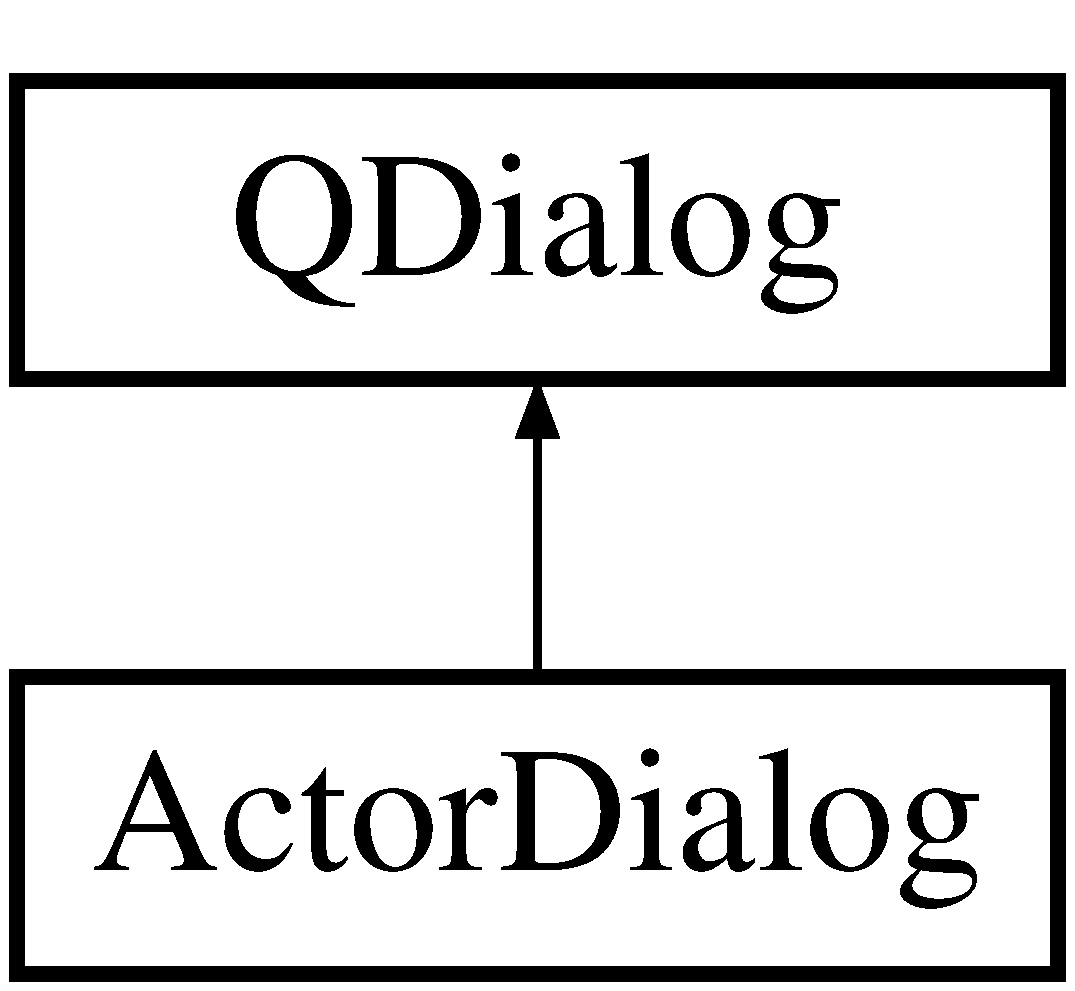
\includegraphics[height=2.000000cm]{class_actor_dialog}
\end{center}
\end{figure}
\subsection*{Public Member Functions}
\begin{DoxyCompactItemize}
\item 
\mbox{\Hypertarget{class_actor_dialog_ab9b196b4e09ea6fd4ad41968fdacc99e}\label{class_actor_dialog_ab9b196b4e09ea6fd4ad41968fdacc99e}} 
{\bfseries Actor\+Dialog} (Q\+Widget $\ast$parent, \hyperlink{class_actor}{Scene\+Actor} $\ast$actor)
\item 
\mbox{\Hypertarget{class_actor_dialog_aef58fd474d7dd8c39d9295fab7f62e5c}\label{class_actor_dialog_aef58fd474d7dd8c39d9295fab7f62e5c}} 
Actor\+Pointer {\bfseries actor} () const
\item 
\mbox{\Hypertarget{class_actor_dialog_a36ecf4e16ca3ca7987fe129079f53bd4}\label{class_actor_dialog_a36ecf4e16ca3ca7987fe129079f53bd4}} 
void {\bfseries actor} (\hyperlink{class_actor}{Scene\+Actor} $\ast$actor)
\item 
\mbox{\Hypertarget{class_actor_dialog_a28986005a09525ecfde09f69740627df}\label{class_actor_dialog_a28986005a09525ecfde09f69740627df}} 
bool {\bfseries ready} () const
\item 
\mbox{\Hypertarget{class_actor_dialog_a2d9c22b6725baf447224d673698ace02}\label{class_actor_dialog_a2d9c22b6725baf447224d673698ace02}} 
void {\bfseries ready} (bool ready)
\end{DoxyCompactItemize}
\subsection*{Private Slots}
\begin{DoxyCompactItemize}
\item 
\mbox{\Hypertarget{class_actor_dialog_a4100201ddb5559e23c285d2f194fcc29}\label{class_actor_dialog_a4100201ddb5559e23c285d2f194fcc29}} 
void {\bfseries action\+Changed} ()
\item 
\mbox{\Hypertarget{class_actor_dialog_ae4e26a1a18ff4514876e524eda5434e4}\label{class_actor_dialog_ae4e26a1a18ff4514876e524eda5434e4}} 
void {\bfseries direction\+Changed} ()
\end{DoxyCompactItemize}
\subsection*{Private Attributes}
\begin{DoxyCompactItemize}
\item 
\mbox{\Hypertarget{class_actor_dialog_a3cb556b9b154afbf22c34f6ea46bce6b}\label{class_actor_dialog_a3cb556b9b154afbf22c34f6ea46bce6b}} 
Ui\+::\+Actor\+Dialog $\ast$ {\bfseries ui}
\item 
\mbox{\Hypertarget{class_actor_dialog_a01865fab8761795a1fcc3a92b37b53e0}\label{class_actor_dialog_a01865fab8761795a1fcc3a92b37b53e0}} 
Actor\+Pointer {\bfseries m\+\_\+actor}
\item 
\mbox{\Hypertarget{class_actor_dialog_a9742ad97f6354534e0edbcc7f34118ae}\label{class_actor_dialog_a9742ad97f6354534e0edbcc7f34118ae}} 
bool {\bfseries m\+\_\+ready}
\end{DoxyCompactItemize}


\subsection{Detailed Description}
The \hyperlink{class_actor_dialog}{Actor\+Dialog} class -\/ defines a dialog box for actor properties. 

The documentation for this class was generated from the following files\+:\begin{DoxyCompactItemize}
\item 
actordialog.\+h\item 
actordialog.\+cpp\end{DoxyCompactItemize}

\hypertarget{class_asset_manager}{}\section{Asset\+Manager Class Reference}
\label{class_asset_manager}\index{Asset\+Manager@{Asset\+Manager}}


The \hyperlink{class_asset_manager}{Asset\+Manager} class -\/ defines a manager for \hyperlink{class_sprite}{Sprite} assets.  




{\ttfamily \#include $<$assetmanager.\+h$>$}

\subsection*{Public Member Functions}
\begin{DoxyCompactItemize}
\item 
\mbox{\Hypertarget{class_asset_manager_af0306dd34eed25aba731bf54a2027193}\label{class_asset_manager_af0306dd34eed25aba731bf54a2027193}} 
{\bfseries Asset\+Manager} (const Q\+String \&name)
\item 
\mbox{\Hypertarget{class_asset_manager_abc08a58cf1fdb77b10e16128ec733c0a}\label{class_asset_manager_abc08a58cf1fdb77b10e16128ec733c0a}} 
Q\+Pixmap {\bfseries get\+Sprite\+Image} (const Q\+String \&page)
\item 
\mbox{\Hypertarget{class_asset_manager_ad40f4a2d968b74c85ba26a377496d0fa}\label{class_asset_manager_ad40f4a2d968b74c85ba26a377496d0fa}} 
Q\+String {\bfseries get\+Sprite\+Sheet\+Name} ()
\item 
\mbox{\Hypertarget{class_asset_manager_a5f5fa8d14fe3711777c83278765a20ff}\label{class_asset_manager_a5f5fa8d14fe3711777c83278765a20ff}} 
Asset\+Map {\bfseries map} ()
\item 
\mbox{\Hypertarget{class_asset_manager_ae7b749953e6c088953213c3f32cbecee}\label{class_asset_manager_ae7b749953e6c088953213c3f32cbecee}} 
Q\+String {\bfseries name} ()
\item 
\mbox{\Hypertarget{class_asset_manager_aebddd385e6cefa6f0e2f940816b57c67}\label{class_asset_manager_aebddd385e6cefa6f0e2f940816b57c67}} 
Coordinates\+Vector {\bfseries image\+\_\+coordinates} (int frame)
\item 
\mbox{\Hypertarget{class_asset_manager_a73b932777ba2543f51304b7fda0b7d5e}\label{class_asset_manager_a73b932777ba2543f51304b7fda0b7d5e}} 
int {\bfseries sprite\+Sheet\+Height} ()
\item 
\mbox{\Hypertarget{class_asset_manager_aa239ebd57768e3eee4422fd0fa75a405}\label{class_asset_manager_aa239ebd57768e3eee4422fd0fa75a405}} 
int {\bfseries sprite\+Sheet\+Width} ()
\item 
\mbox{\Hypertarget{class_asset_manager_a629953081d689b6ce4ae68c86ba292cf}\label{class_asset_manager_a629953081d689b6ce4ae68c86ba292cf}} 
int {\bfseries sprite\+Sheet\+Columns} ()
\item 
\mbox{\Hypertarget{class_asset_manager_ae7df2f180d987957d1b28959ba39643d}\label{class_asset_manager_ae7df2f180d987957d1b28959ba39643d}} 
int {\bfseries sprite\+Sheet\+Rows} ()
\item 
\mbox{\Hypertarget{class_asset_manager_aa3161c0ad9ac8dbab9d8732a47335f22}\label{class_asset_manager_aa3161c0ad9ac8dbab9d8732a47335f22}} 
int {\bfseries sprite\+Width} ()
\item 
\mbox{\Hypertarget{class_asset_manager_ab800356c8b05a8fed62e522a3cea11d9}\label{class_asset_manager_ab800356c8b05a8fed62e522a3cea11d9}} 
int {\bfseries sprite\+Height} ()
\item 
\mbox{\Hypertarget{class_asset_manager_a716db89db2e5cf1405d3cf3906f581b7}\label{class_asset_manager_a716db89db2e5cf1405d3cf3906f581b7}} 
int {\bfseries sprite\+Page\+Row} (const Q\+String \&)
\item 
\mbox{\Hypertarget{class_asset_manager_a554a984f9edbac3fd4b2a52e983ea74d}\label{class_asset_manager_a554a984f9edbac3fd4b2a52e983ea74d}} 
int {\bfseries sprite\+Page\+Col} (const Q\+String \&page)
\item 
\mbox{\Hypertarget{class_asset_manager_abe76754e3b6a55d19969772a12dd42f8}\label{class_asset_manager_abe76754e3b6a55d19969772a12dd42f8}} 
int {\bfseries sprite\+Page\+Columns} (const Q\+String \&name)
\item 
\mbox{\Hypertarget{class_asset_manager_a577dacd1b7f1631f808fe7c68c4638de}\label{class_asset_manager_a577dacd1b7f1631f808fe7c68c4638de}} 
Q\+Json\+Array {\bfseries actor\+Friends} ()
\item 
\mbox{\Hypertarget{class_asset_manager_ac0d791cc43c7dd68fd8ff43fb69a3619}\label{class_asset_manager_ac0d791cc43c7dd68fd8ff43fb69a3619}} 
Q\+Json\+Array {\bfseries actor\+Foes} ()
\item 
\mbox{\Hypertarget{class_asset_manager_a98e88dbd0bdc8e409d13815556071a2a}\label{class_asset_manager_a98e88dbd0bdc8e409d13815556071a2a}} 
Q\+Json\+Array {\bfseries actor\+Actions} ()
\item 
\mbox{\Hypertarget{class_asset_manager_afbd4c4a3edfef4a4d7fe68e1a1953a2c}\label{class_asset_manager_afbd4c4a3edfef4a4d7fe68e1a1953a2c}} 
Q\+Json\+Array {\bfseries actor\+Direction\+Set} ()
\item 
\mbox{\Hypertarget{class_asset_manager_ab114e7886b4de3519590f913f508706a}\label{class_asset_manager_ab114e7886b4de3519590f913f508706a}} 
Q\+String {\bfseries actor\+Primary\+Fight\+Action} ()
\item 
\mbox{\Hypertarget{class_asset_manager_a2c2b23679fe2e0e736e12beeaae99198}\label{class_asset_manager_a2c2b23679fe2e0e736e12beeaae99198}} 
bool {\bfseries has\+Action} (const Q\+String \&name)
\end{DoxyCompactItemize}
\subsection*{Private Member Functions}
\begin{DoxyCompactItemize}
\item 
void \hyperlink{class_asset_manager_aa1d50ebdf4aa6df6fba090e649eb6ec0}{init} (const Q\+String \&name)
\begin{DoxyCompactList}\small\item\em \hyperlink{class_asset_manager_aa1d50ebdf4aa6df6fba090e649eb6ec0}{Asset\+Manager\+::init} -\/ initialize the asset manager. \end{DoxyCompactList}\end{DoxyCompactItemize}
\subsection*{Private Attributes}
\begin{DoxyCompactItemize}
\item 
\mbox{\Hypertarget{class_asset_manager_a64d1471c74b7bcd96ebc04e4a3458d54}\label{class_asset_manager_a64d1471c74b7bcd96ebc04e4a3458d54}} 
Q\+String {\bfseries m\+\_\+name}
\item 
\mbox{\Hypertarget{class_asset_manager_af8c2ecb2870be050880deed6d55f5332}\label{class_asset_manager_af8c2ecb2870be050880deed6d55f5332}} 
Coordinates\+Vector {\bfseries m\+\_\+sprite\+\_\+image\+\_\+coordinates}
\end{DoxyCompactItemize}
\subsection*{Static Private Attributes}
\begin{DoxyCompactItemize}
\item 
\mbox{\Hypertarget{class_asset_manager_a8c7dee0564fcd582ae15c299afa758f2}\label{class_asset_manager_a8c7dee0564fcd582ae15c299afa758f2}} 
static Asset\+Map {\bfseries m\+\_\+asset\+\_\+map}
\end{DoxyCompactItemize}


\subsection{Detailed Description}
The \hyperlink{class_asset_manager}{Asset\+Manager} class -\/ defines a manager for \hyperlink{class_sprite}{Sprite} assets. 

\subsection{Member Function Documentation}
\mbox{\Hypertarget{class_asset_manager_aa1d50ebdf4aa6df6fba090e649eb6ec0}\label{class_asset_manager_aa1d50ebdf4aa6df6fba090e649eb6ec0}} 
\index{Asset\+Manager@{Asset\+Manager}!init@{init}}
\index{init@{init}!Asset\+Manager@{Asset\+Manager}}
\subsubsection{\texorpdfstring{init()}{init()}}
{\footnotesize\ttfamily void Asset\+Manager\+::init (\begin{DoxyParamCaption}\item[{const Q\+String \&}]{name }\end{DoxyParamCaption})\hspace{0.3cm}{\ttfamily [private]}}



\hyperlink{class_asset_manager_aa1d50ebdf4aa6df6fba090e649eb6ec0}{Asset\+Manager\+::init} -\/ initialize the asset manager. 


\begin{DoxyParams}{Parameters}
{\em name} & \\
\hline
\end{DoxyParams}

\begin{DoxyCode}
17                                            \{
18     QString settings;
19     QFile file;
20     file.setFileName(\textcolor{stringliteral}{":/config/characters/"}+name+\textcolor{stringliteral}{".json"});
21     file.open(QIODevice::ReadOnly | QIODevice::Text);
22     settings = file.readAll();
23     file.close();
24     QJsonDocument sd = QJsonDocument::fromJson(settings.toUtf8());
25     \textcolor{keywordflow}{if}(sd.isEmpty()) \{
26         \textcolor{keywordflow}{throw} \textcolor{stringliteral}{"Error with JSON Document: "} + name + \textcolor{stringliteral}{".json"};
27     \}
28     QJsonObject sett2 = sd.object();
29     m\_asset\_map[name+\textcolor{stringliteral}{"\_sprite\_sheet\_name"}] = sett2[\textcolor{stringliteral}{"spritesheet"}].toString();
30     m\_asset\_map[name+\textcolor{stringliteral}{"\_friends"}] = sett2[\textcolor{stringliteral}{"friends"}].toArray();
31     m\_asset\_map[name+\textcolor{stringliteral}{"\_foes"}] = sett2[\textcolor{stringliteral}{"foes"}].toArray();
32     m\_asset\_map[name+\textcolor{stringliteral}{"\_actions"}] = sett2[\textcolor{stringliteral}{"actions"}].toArray();
33     m\_asset\_map[name+\textcolor{stringliteral}{"\_directions"}] = sett2[\textcolor{stringliteral}{"directions"}].toArray();
34     m\_asset\_map[name+\textcolor{stringliteral}{"\_primary\_fight\_action"}] = sett2[\textcolor{stringliteral}{"primary\_fight\_action"}].toString();
35     m\_asset\_map[name+\textcolor{stringliteral}{"\_default"}] = QPixmap(sett2[\textcolor{stringliteral}{"spritesheet"}].toString());
36     QVariantMap imp = sett2[\textcolor{stringliteral}{"image\_properties"}].toVariant().toMap();
37     \textcolor{keywordflow}{for}(\textcolor{keyword}{auto} key : imp.keys()) \{
38         m\_asset\_map[name+\textcolor{stringliteral}{"\_image\_properties\_"}+key] = imp[key].value<\textcolor{keywordtype}{int}>();
39     \}
40     m\_asset\_map[name+\textcolor{stringliteral}{"\_image\_properties"}] = sett2[\textcolor{stringliteral}{"image\_properties"}].toVariant().toMap();
41     QVariantMap m = sett2[\textcolor{stringliteral}{"sprite\_pages"}].toVariant().toMap();
42     \textcolor{keywordflow}{for}(\textcolor{keyword}{auto} key : m.keys()) \{
43         m\_asset\_map[name+\textcolor{stringliteral}{"\_sprite\_"}+key+\textcolor{stringliteral}{"\_row"}] = m[key].value<QVariantMap>()[\textcolor{stringliteral}{"row"}].value<int>();
44         m\_asset\_map[name+\textcolor{stringliteral}{"\_sprite\_"}+key+\textcolor{stringliteral}{"\_col"}] = m[key].value<QVariantMap>()[\textcolor{stringliteral}{"col"}].value<int>();
45         m\_asset\_map[name+\textcolor{stringliteral}{"\_sprite\_"}+key+\textcolor{stringliteral}{"\_cells"}] = m[key].value<QVariantMap>()[\textcolor{stringliteral}{"cells"}].value<int>();
46     \}
47 \}
\end{DoxyCode}


The documentation for this class was generated from the following files\+:\begin{DoxyCompactItemize}
\item 
assetmanager.\+h\item 
assetmanager.\+cpp\end{DoxyCompactItemize}

\hypertarget{class_console_widget}{}\section{Console\+Widget Class Reference}
\label{class_console_widget}\index{Console\+Widget@{Console\+Widget}}


The \hyperlink{class_console_widget}{Console\+Widget} class -- Provides a console for use in a \hyperlink{class_game_scene}{Game\+Scene}.  




{\ttfamily \#include $<$consolewidget.\+h$>$}

Inheritance diagram for Console\+Widget\+:\begin{figure}[H]
\begin{center}
\leavevmode
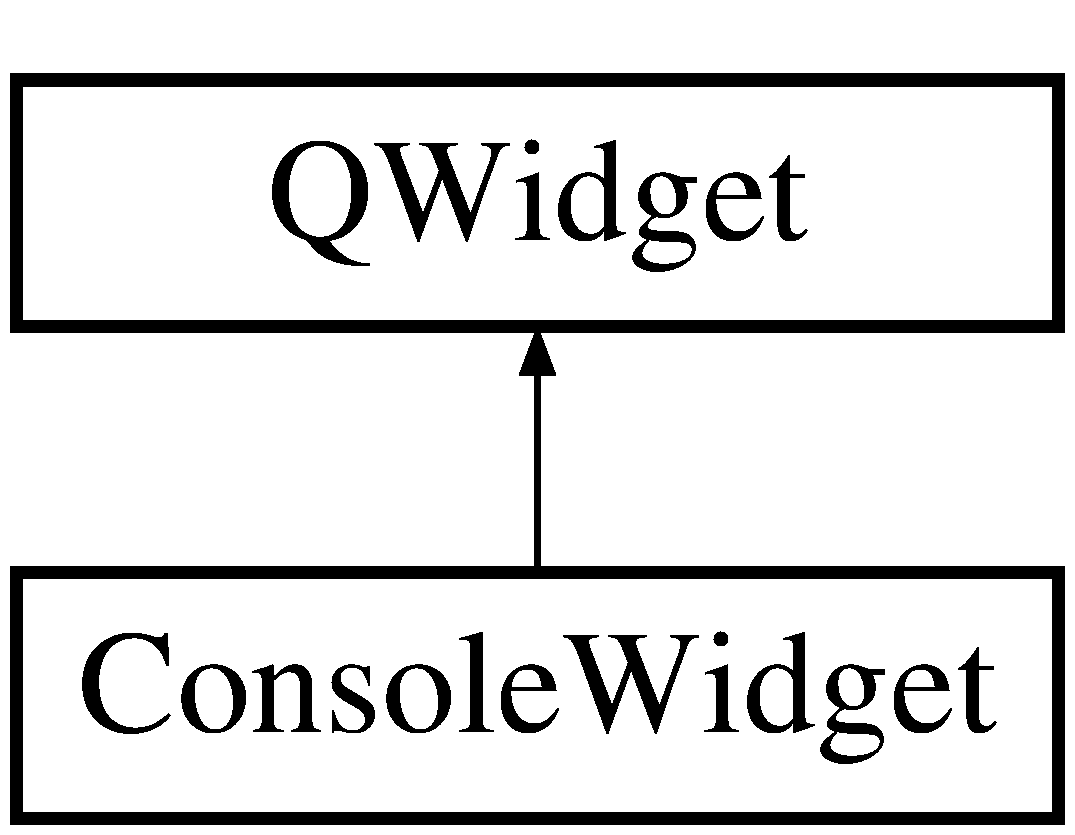
\includegraphics[height=2.000000cm]{class_console_widget}
\end{center}
\end{figure}
\subsection*{Public Slots}
\begin{DoxyCompactItemize}
\item 
\mbox{\Hypertarget{class_console_widget_a25c9db0a82f572647288b738f1b1781d}\label{class_console_widget_a25c9db0a82f572647288b738f1b1781d}} 
void {\bfseries send\+Text} ()
\end{DoxyCompactItemize}
\subsection*{Signals}
\begin{DoxyCompactItemize}
\item 
\mbox{\Hypertarget{class_console_widget_a5ff85011eea230aefe8633b329d5132f}\label{class_console_widget_a5ff85011eea230aefe8633b329d5132f}} 
void {\bfseries signal\+Text} (const char $\ast$)
\end{DoxyCompactItemize}
\subsection*{Public Member Functions}
\begin{DoxyCompactItemize}
\item 
\mbox{\Hypertarget{class_console_widget_a4a66caaf3f7583a46ebe44a5c2221160}\label{class_console_widget_a4a66caaf3f7583a46ebe44a5c2221160}} 
{\bfseries Console\+Widget} (Q\+Widget $\ast$parent=0)
\item 
\mbox{\Hypertarget{class_console_widget_a599f0a9577aa0f63e3aad3714de14925}\label{class_console_widget_a599f0a9577aa0f63e3aad3714de14925}} 
Q\+Text\+Edit $\ast$ {\bfseries textedit} () const
\end{DoxyCompactItemize}
\subsection*{Private Attributes}
\begin{DoxyCompactItemize}
\item 
\mbox{\Hypertarget{class_console_widget_a8a1debe1a354c1d403b1deea7c25a0aa}\label{class_console_widget_a8a1debe1a354c1d403b1deea7c25a0aa}} 
Q\+Text\+Edit $\ast$ {\bfseries m\+\_\+textedit}
\end{DoxyCompactItemize}


\subsection{Detailed Description}
The \hyperlink{class_console_widget}{Console\+Widget} class -- Provides a console for use in a \hyperlink{class_game_scene}{Game\+Scene}. 

The documentation for this class was generated from the following files\+:\begin{DoxyCompactItemize}
\item 
consolewidget.\+h\item 
consolewidget.\+cpp\end{DoxyCompactItemize}

\hypertarget{classmfg_1_1_engine}{}\section{mfg\+:\+:Engine Class Reference}
\label{classmfg_1_1_engine}\index{mfg\+::\+Engine@{mfg\+::\+Engine}}


The \hyperlink{classmfg_1_1_engine}{Engine} class -\/ a game engine.  




{\ttfamily \#include $<$gameengine.\+h$>$}

\subsection*{Public Member Functions}
\begin{DoxyCompactItemize}
\item 
\mbox{\Hypertarget{classmfg_1_1_engine_a687d0b7b9c5744312b52925cc365249e}\label{classmfg_1_1_engine_a687d0b7b9c5744312b52925cc365249e}} 
Q\+Script\+Engine $\ast$ {\bfseries scriptengine} ()
\item 
\mbox{\Hypertarget{classmfg_1_1_engine_a70efe8bcf90b5ffc41cbf3e3e11f1e19}\label{classmfg_1_1_engine_a70efe8bcf90b5ffc41cbf3e3e11f1e19}} 
Q\+Url {\bfseries audio\+File} (const Q\+String \&file)
\item 
\mbox{\Hypertarget{classmfg_1_1_engine_a268d9d9bf7bed17b80c0bd22bffd4d8c}\label{classmfg_1_1_engine_a268d9d9bf7bed17b80c0bd22bffd4d8c}} 
\hyperlink{structmfg_1_1_stats}{Stats} {\bfseries get\+Default\+Stats} (const Q\+String \&name)
\item 
\mbox{\Hypertarget{classmfg_1_1_engine_a64ff2b62c87bd742495c1bbd11c1dba5}\label{classmfg_1_1_engine_a64ff2b62c87bd742495c1bbd11c1dba5}} 
int {\bfseries max\+\_\+life} (const Q\+String \&name) const
\item 
\mbox{\Hypertarget{classmfg_1_1_engine_a5618e671129e7689e59a139be9dd1c3a}\label{classmfg_1_1_engine_a5618e671129e7689e59a139be9dd1c3a}} 
void {\bfseries build\+Actor\+Rules} ()
\item 
\mbox{\Hypertarget{classmfg_1_1_engine_a54ac63e738b56fcebde8b938f6564d37}\label{classmfg_1_1_engine_a54ac63e738b56fcebde8b938f6564d37}} 
void {\bfseries build\+Asset\+Map} ()
\item 
\mbox{\Hypertarget{classmfg_1_1_engine_aab8b2f5a5ef432825a3973e839a24d78}\label{classmfg_1_1_engine_aab8b2f5a5ef432825a3973e839a24d78}} 
void {\bfseries build\+Pixmaps} ()
\item 
\mbox{\Hypertarget{classmfg_1_1_engine_af0d7f38782bda7e1582ca7b8605fdd63}\label{classmfg_1_1_engine_af0d7f38782bda7e1582ca7b8605fdd63}} 
\hyperlink{class_asset_manager}{Asset\+Manager} $\ast$ {\bfseries add\+Asset\+Manager} (const Q\+String \&name, \hyperlink{class_asset_manager}{Asset\+Manager} $\ast$am)
\item 
\mbox{\Hypertarget{classmfg_1_1_engine_a2add7951cfef6093f77d07c7780d4def}\label{classmfg_1_1_engine_a2add7951cfef6093f77d07c7780d4def}} 
\hyperlink{class_asset_manager}{Asset\+Manager} $\ast$ {\bfseries asset\+Manager} (const Q\+String \&name)
\item 
\mbox{\Hypertarget{classmfg_1_1_engine_a57372977f9e802e67a9f7bce0cd983e7}\label{classmfg_1_1_engine_a57372977f9e802e67a9f7bce0cd983e7}} 
\hyperlink{class_rule_set}{Rule\+Set} $\ast$ {\bfseries rule\+Factory} (const Q\+String \&name)
\item 
\mbox{\Hypertarget{classmfg_1_1_engine_a3bd604d0698f7e72c38051cdeaff10d2}\label{classmfg_1_1_engine_a3bd604d0698f7e72c38051cdeaff10d2}} 
\hyperlink{class_rule_set}{Rule\+Set} $\ast$ {\bfseries actor\+Rule} (const Q\+String \&name)
\item 
\mbox{\Hypertarget{classmfg_1_1_engine_a3a06b7886658de0da68ca942a0b837b0}\label{classmfg_1_1_engine_a3a06b7886658de0da68ca942a0b837b0}} 
\hyperlink{class_rule_set}{Rule\+Set} $\ast$ {\bfseries add\+Actor\+Rule} (const Q\+String \&name, \hyperlink{class_rule_set}{Rule\+Set} $\ast$rule)
\item 
\mbox{\Hypertarget{classmfg_1_1_engine_a2467edce40ee2d41b688d047df2396b0}\label{classmfg_1_1_engine_a2467edce40ee2d41b688d047df2396b0}} 
Q\+Pixmap $\ast$ {\bfseries add\+Pixmap} (const Q\+String \&name, Q\+Pixmap $\ast$pm)
\item 
\mbox{\Hypertarget{classmfg_1_1_engine_ad212205e8b53041f1284013ff4a7eacb}\label{classmfg_1_1_engine_ad212205e8b53041f1284013ff4a7eacb}} 
Q\+Pixmap $\ast$ {\bfseries pix\+Map} (const Q\+String \&name)
\item 
\mbox{\Hypertarget{classmfg_1_1_engine_a6ef9267c4fc390f42ae27baef1c6f701}\label{classmfg_1_1_engine_a6ef9267c4fc390f42ae27baef1c6f701}} 
Rule\+Map {\bfseries get\+Actor\+\_\+rules} () const
\item 
\mbox{\Hypertarget{classmfg_1_1_engine_aacf5e27746b15291536e0573cfc4e415}\label{classmfg_1_1_engine_aacf5e27746b15291536e0573cfc4e415}} 
void {\bfseries set\+Actor\+\_\+rules} (const Rule\+Map \&player\+\_\+rules)
\item 
\mbox{\Hypertarget{classmfg_1_1_engine_af4126c00eb8ac07bd8bc56f67f4b0890}\label{classmfg_1_1_engine_af4126c00eb8ac07bd8bc56f67f4b0890}} 
Q\+Media\+Player $\ast$ {\bfseries mediaplayer} () const
\item 
\mbox{\Hypertarget{classmfg_1_1_engine_ae9401d26bc77d69553e9d4d58bc7ce22}\label{classmfg_1_1_engine_ae9401d26bc77d69553e9d4d58bc7ce22}} 
void {\bfseries set\+Media\+Player} (Q\+Media\+Player $\ast$player)
\item 
\mbox{\Hypertarget{classmfg_1_1_engine_a8d31d4eb54252e8523775f8dff145a92}\label{classmfg_1_1_engine_a8d31d4eb54252e8523775f8dff145a92}} 
Q\+Media\+Playlist $\ast$ {\bfseries mediaplaylist} () const
\item 
\mbox{\Hypertarget{classmfg_1_1_engine_a296fdd5e8062a6cb7214bb3a44bc70e6}\label{classmfg_1_1_engine_a296fdd5e8062a6cb7214bb3a44bc70e6}} 
void {\bfseries set\+Playlist} (Q\+Media\+Playlist $\ast$playlist)
\item 
\mbox{\Hypertarget{classmfg_1_1_engine_acba63454459c76adbea96bc609669491}\label{classmfg_1_1_engine_acba63454459c76adbea96bc609669491}} 
\hyperlink{class_scene_manager}{Scene\+Manager} $\ast$ {\bfseries scene\+Manager} () const
\item 
\mbox{\Hypertarget{classmfg_1_1_engine_ac673b51dbad9a39968d1e5a57c92b040}\label{classmfg_1_1_engine_ac673b51dbad9a39968d1e5a57c92b040}} 
void {\bfseries set\+Scene\+Manager} (\hyperlink{class_scene_manager}{Scene\+Manager} $\ast$scene\+Manager)
\end{DoxyCompactItemize}
\subsection*{Static Public Member Functions}
\begin{DoxyCompactItemize}
\item 
\mbox{\Hypertarget{classmfg_1_1_engine_a826e8e5359c8f5f2516fb7e4ad8ae3a0}\label{classmfg_1_1_engine_a826e8e5359c8f5f2516fb7e4ad8ae3a0}} 
static Q\+Vector$<$ Q\+String $>$ {\bfseries actors} ()
\end{DoxyCompactItemize}
\subsection*{Private Attributes}
\begin{DoxyCompactItemize}
\item 
\mbox{\Hypertarget{classmfg_1_1_engine_ad2401d178403008525cfd6a1caa85ae5}\label{classmfg_1_1_engine_ad2401d178403008525cfd6a1caa85ae5}} 
Q\+Script\+Engine $\ast$ {\bfseries m\+\_\+script\+\_\+engine}
\item 
\mbox{\Hypertarget{classmfg_1_1_engine_a24bac160b2daf5247d6b5d70499311f6}\label{classmfg_1_1_engine_a24bac160b2daf5247d6b5d70499311f6}} 
\hyperlink{class_scene_manager}{Scene\+Manager} $\ast$ {\bfseries m\+\_\+scene\+\_\+manager}
\item 
\mbox{\Hypertarget{classmfg_1_1_engine_a8b648c4f7a59c9993a30179b4711c92b}\label{classmfg_1_1_engine_a8b648c4f7a59c9993a30179b4711c92b}} 
Rule\+Map {\bfseries m\+\_\+actor\+\_\+rules}
\item 
\mbox{\Hypertarget{classmfg_1_1_engine_a18f50fe08592b70969ff6c8113f18753}\label{classmfg_1_1_engine_a18f50fe08592b70969ff6c8113f18753}} 
Asset\+Manager\+Map {\bfseries m\+\_\+assets}
\item 
\mbox{\Hypertarget{classmfg_1_1_engine_ab9813b744a07242fc2a3adc7d796cd20}\label{classmfg_1_1_engine_ab9813b744a07242fc2a3adc7d796cd20}} 
Pixmap\+Map {\bfseries m\+\_\+pixmaps}
\item 
\mbox{\Hypertarget{classmfg_1_1_engine_ac423142f783829c549531219290966e2}\label{classmfg_1_1_engine_ac423142f783829c549531219290966e2}} 
Q\+Media\+Player $\ast$ {\bfseries m\+\_\+player}
\item 
\mbox{\Hypertarget{classmfg_1_1_engine_ae6f5890f6e9a33a6891957e671fbf41c}\label{classmfg_1_1_engine_ae6f5890f6e9a33a6891957e671fbf41c}} 
Q\+Media\+Playlist $\ast$ {\bfseries m\+\_\+playlist}
\end{DoxyCompactItemize}


\subsection{Detailed Description}
The \hyperlink{classmfg_1_1_engine}{Engine} class -\/ a game engine. 

The documentation for this class was generated from the following files\+:\begin{DoxyCompactItemize}
\item 
gameengine.\+h\item 
gameengine.\+cpp\end{DoxyCompactItemize}

\hypertarget{class_game_scene}{}\section{Game\+Scene Class Reference}
\label{class_game_scene}\index{Game\+Scene@{Game\+Scene}}


The \hyperlink{class_game_scene}{Game\+Scene} class -\/ creates a graphic scene used for game play.  




{\ttfamily \#include $<$gamescene.\+h$>$}

Inheritance diagram for Game\+Scene\+:\begin{figure}[H]
\begin{center}
\leavevmode
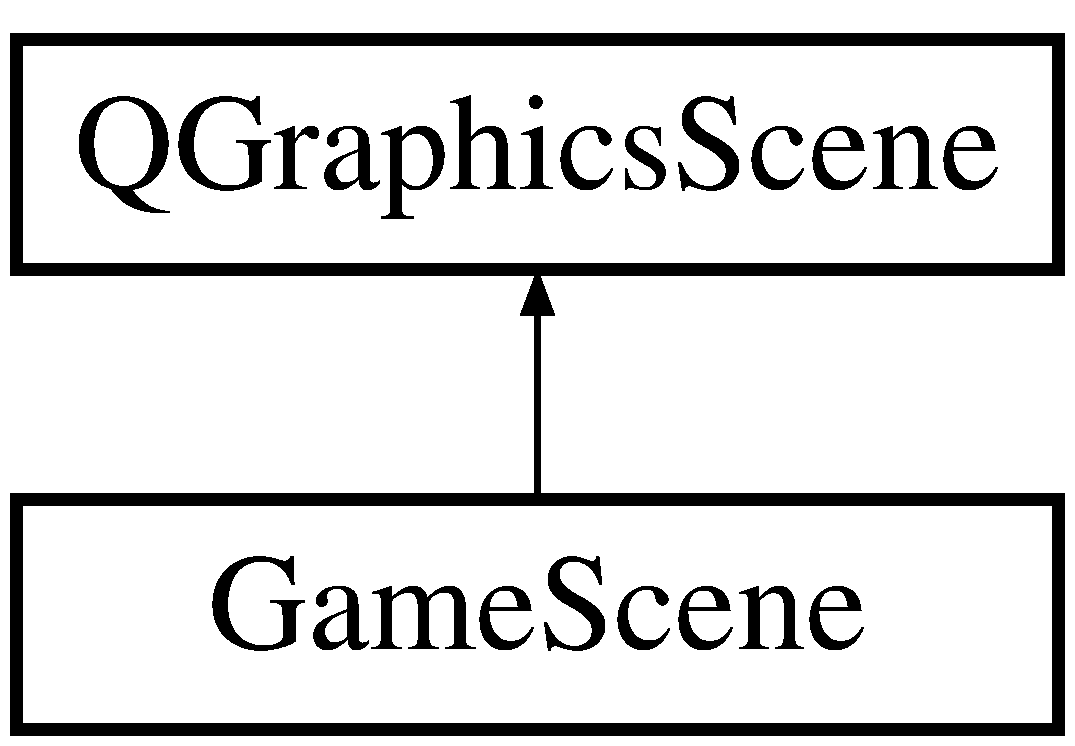
\includegraphics[height=2.000000cm]{class_game_scene}
\end{center}
\end{figure}
\subsection*{Public Slots}
\begin{DoxyCompactItemize}
\item 
\mbox{\Hypertarget{class_game_scene_a5eaeebac1ab47bc9cb51dba7273f787d}\label{class_game_scene_a5eaeebac1ab47bc9cb51dba7273f787d}} 
void {\bfseries sprite\+Selected} (Q\+Graphics\+Scene\+Mouse\+Event $\ast$, \hyperlink{class_sprite}{Sprite} $\ast$)
\item 
\mbox{\Hypertarget{class_game_scene_a54b85a8a3edf7109043576175845cae0}\label{class_game_scene_a54b85a8a3edf7109043576175845cae0}} 
void {\bfseries advance} ()
\item 
\mbox{\Hypertarget{class_game_scene_ad692069ae30670af3c614c0b783622f3}\label{class_game_scene_ad692069ae30670af3c614c0b783622f3}} 
void {\bfseries actor\+Collision} ()
\end{DoxyCompactItemize}
\subsection*{Public Member Functions}
\begin{DoxyCompactItemize}
\item 
\mbox{\Hypertarget{class_game_scene_abf292a17082d258a7c9a670c2eda50ea}\label{class_game_scene_abf292a17082d258a7c9a670c2eda50ea}} 
{\bfseries Game\+Scene} (\hyperlink{class_scene_manager}{Scene\+Manager} $\ast$sm, Q\+Object $\ast$parent=0, const Q\+RectF \&rect=Q\+RectF(-\/300,-\/300, 600, 600))
\item 
\mbox{\Hypertarget{class_game_scene_a02a45a8bd424e6a09fb928b84abab216}\label{class_game_scene_a02a45a8bd424e6a09fb928b84abab216}} 
void {\bfseries connect\+Timer} (Q\+Timer $\ast$)
\item 
\mbox{\Hypertarget{class_game_scene_a5472c7fdab73c3f2633861a2fc77fdfc}\label{class_game_scene_a5472c7fdab73c3f2633861a2fc77fdfc}} 
void {\bfseries add\+Item} (Q\+Graphics\+Item $\ast$item, const Q\+String \&name)
\item 
\mbox{\Hypertarget{class_game_scene_a51c98b3db623b2247afa8b6360d4a04b}\label{class_game_scene_a51c98b3db623b2247afa8b6360d4a04b}} 
\hyperlink{class_actor}{Scene\+Actor} $\ast$ {\bfseries add\+Actor} (const Q\+String \&name, const Q\+String \&start\+\_\+action, bool moving)
\item 
\mbox{\Hypertarget{class_game_scene_adfa6afce903509fba5324dd822365937}\label{class_game_scene_adfa6afce903509fba5324dd822365937}} 
\hyperlink{class_sprite}{Sprite} $\ast$ {\bfseries add\+Sprite} (const Q\+String \&name, const Q\+String \&start\+\_\+action, bool moving)
\item 
\mbox{\Hypertarget{class_game_scene_a9ce725296c40edfad55477389d771b5a}\label{class_game_scene_a9ce725296c40edfad55477389d771b5a}} 
void {\bfseries remove\+Actor} (\hyperlink{class_actor}{Scene\+Actor} $\ast$)
\item 
\mbox{\Hypertarget{class_game_scene_a7c837f21ae8de156ffe364f61512126d}\label{class_game_scene_a7c837f21ae8de156ffe364f61512126d}} 
\hyperlink{class_sprite}{Sprite} $\ast$ {\bfseries current\+\_\+sprite} ()
\item 
\mbox{\Hypertarget{class_game_scene_a583bc8b9dbeb21d89be15c1e9af85898}\label{class_game_scene_a583bc8b9dbeb21d89be15c1e9af85898}} 
\hyperlink{class_sprite}{Sprite} $\ast$ {\bfseries current\+\_\+sprite} (\hyperlink{class_sprite}{Sprite} $\ast$)
\item 
\mbox{\Hypertarget{class_game_scene_a748a3207ff433972a6ea24d2dbbb089d}\label{class_game_scene_a748a3207ff433972a6ea24d2dbbb089d}} 
Actor\+Count\+Map {\bfseries get\+Actor\+Counts} ()
\item 
\mbox{\Hypertarget{class_game_scene_a13d54b44f642489278e20b486678c686}\label{class_game_scene_a13d54b44f642489278e20b486678c686}} 
Actor\+List {\bfseries get\+All\+Actors} ()
\item 
\mbox{\Hypertarget{class_game_scene_a8a811a7b2497a20b8e0757e2bdc26932}\label{class_game_scene_a8a811a7b2497a20b8e0757e2bdc26932}} 
Q\+Vector$<$ Q\+String $>$ {\bfseries players} ()
\item 
\mbox{\Hypertarget{class_game_scene_a7077ce88eca56dee27ba8deae2c5c1bf}\label{class_game_scene_a7077ce88eca56dee27ba8deae2c5c1bf}} 
int {\bfseries dead\+Count} ()
\item 
\mbox{\Hypertarget{class_game_scene_a26ee4d4610a8fd5b9af762d8a3c2f8d7}\label{class_game_scene_a26ee4d4610a8fd5b9af762d8a3c2f8d7}} 
void {\bfseries clear\+Dead} ()
\item 
\mbox{\Hypertarget{class_game_scene_aeb498f64c57482b7a340587c03f886d9}\label{class_game_scene_aeb498f64c57482b7a340587c03f886d9}} 
bool {\bfseries is\+Scene\+Actor} (Q\+Graphics\+Item $\ast$item)
\item 
\mbox{\Hypertarget{class_game_scene_aa55dfeaf2d458b5c05d4dc206f8022ed}\label{class_game_scene_aa55dfeaf2d458b5c05d4dc206f8022ed}} 
void {\bfseries clear\+Actors} ()
\item 
\mbox{\Hypertarget{class_game_scene_a6971c7adf7fed708c747322324ee2045}\label{class_game_scene_a6971c7adf7fed708c747322324ee2045}} 
Graphics\+Item\+List {\bfseries get\+Deadlist} () const
\item 
\mbox{\Hypertarget{class_game_scene_a18424ff3ed1d4c423a7ca20f2191983c}\label{class_game_scene_a18424ff3ed1d4c423a7ca20f2191983c}} 
void {\bfseries set\+Deadlist} (const Graphics\+Item\+List \&deadlist)
\item 
\mbox{\Hypertarget{class_game_scene_a484d473ed3a7537aec18066a382480d2}\label{class_game_scene_a484d473ed3a7537aec18066a382480d2}} 
Q\+Time {\bfseries current\+\_\+time} ()
\item 
\mbox{\Hypertarget{class_game_scene_ac5875684ca060591cad3f2e02c3c7a21}\label{class_game_scene_ac5875684ca060591cad3f2e02c3c7a21}} 
Q\+Graphics\+Item $\ast$ {\bfseries set\+Background\+Image\+By\+Name} (const Q\+String \&name)
\item 
\mbox{\Hypertarget{class_game_scene_a0d67003cada8079ada8c2bf7ea924134}\label{class_game_scene_a0d67003cada8079ada8c2bf7ea924134}} 
\hyperlink{classmfg_1_1_engine}{mfg\+::\+Engine} $\ast$ {\bfseries game\+Engine} ()
\item 
\mbox{\Hypertarget{class_game_scene_a774aaa53865ee6184b3bbcec5ed976b0}\label{class_game_scene_a774aaa53865ee6184b3bbcec5ed976b0}} 
\hyperlink{class_console_widget}{Console\+Widget} $\ast$ {\bfseries console} ()
\item 
\mbox{\Hypertarget{class_game_scene_ac0fedd57d4e9d653803b27fd62485211}\label{class_game_scene_ac0fedd57d4e9d653803b27fd62485211}} 
\hyperlink{class_scene_manager}{Scene\+Manager} $\ast$ {\bfseries scene\+Manager} () const
\item 
\mbox{\Hypertarget{class_game_scene_a415fd6b00796cce9ac40618e3f94db4b}\label{class_game_scene_a415fd6b00796cce9ac40618e3f94db4b}} 
void {\bfseries scene\+Manager} (\hyperlink{class_scene_manager}{Scene\+Manager} $\ast$scene\+Manager)
\item 
\mbox{\Hypertarget{class_game_scene_a2f075555a06267a4e150506c423846b0}\label{class_game_scene_a2f075555a06267a4e150506c423846b0}} 
Q\+Timer $\ast$ {\bfseries timer} ()
\item 
\mbox{\Hypertarget{class_game_scene_a0fd4969df4e5f5f635f9ab5d3e66c404}\label{class_game_scene_a0fd4969df4e5f5f635f9ab5d3e66c404}} 
Q\+String {\bfseries name} () const
\item 
\mbox{\Hypertarget{class_game_scene_a6eb8d5be7ee8f1ebb50a7fd49e9c2a35}\label{class_game_scene_a6eb8d5be7ee8f1ebb50a7fd49e9c2a35}} 
void {\bfseries set\+Name} (const Q\+String \&name)
\end{DoxyCompactItemize}
\subsection*{Protected Slots}
\begin{DoxyCompactItemize}
\item 
void \hyperlink{class_game_scene_a60e084f3ade89e765a5ff86f2c0d7bf1}{mouse\+Move\+Event} (Q\+Graphics\+Scene\+Mouse\+Event $\ast$mouse\+Event) override
\end{DoxyCompactItemize}
\subsection*{Private Attributes}
\begin{DoxyCompactItemize}
\item 
\mbox{\Hypertarget{class_game_scene_a962b8138354a26715c566c51766dba50}\label{class_game_scene_a962b8138354a26715c566c51766dba50}} 
Q\+String {\bfseries m\+\_\+name}
\item 
\mbox{\Hypertarget{class_game_scene_a028e0e563ec3bd30a9afb606ef75e9f7}\label{class_game_scene_a028e0e563ec3bd30a9afb606ef75e9f7}} 
\hyperlink{class_sprite}{Sprite} $\ast$ {\bfseries m\+\_\+current\+\_\+sprite}
\item 
\mbox{\Hypertarget{class_game_scene_ad2ccaf177a7647a85c3a7cdbdd646fb8}\label{class_game_scene_ad2ccaf177a7647a85c3a7cdbdd646fb8}} 
\hyperlink{classmfg_1_1_engine}{mfg\+::\+Engine} $\ast$ {\bfseries m\+\_\+game\+\_\+engine}
\item 
\mbox{\Hypertarget{class_game_scene_a9caa2f44e6b54ab2e2e1278856b05503}\label{class_game_scene_a9caa2f44e6b54ab2e2e1278856b05503}} 
\hyperlink{class_scene_manager}{Scene\+Manager} $\ast$ {\bfseries m\+\_\+scene\+\_\+manager}
\item 
\mbox{\Hypertarget{class_game_scene_af7f8cdc994102b36ddf0e6cf473859e2}\label{class_game_scene_af7f8cdc994102b36ddf0e6cf473859e2}} 
Graphics\+Item\+List {\bfseries m\+\_\+deadlist}
\item 
\mbox{\Hypertarget{class_game_scene_afd3b6181bf71e4928c819cef61d3e246}\label{class_game_scene_afd3b6181bf71e4928c819cef61d3e246}} 
Q\+Time {\bfseries m\+\_\+current\+\_\+time}
\item 
\mbox{\Hypertarget{class_game_scene_a46a12d66c156b32129df54d08e4afea8}\label{class_game_scene_a46a12d66c156b32129df54d08e4afea8}} 
Q\+Timer $\ast$ {\bfseries m\+\_\+timer}
\item 
\mbox{\Hypertarget{class_game_scene_abda4ce287b680ead5be56d31712d6d17}\label{class_game_scene_abda4ce287b680ead5be56d31712d6d17}} 
\hyperlink{class_console_widget}{Console\+Widget} $\ast$ {\bfseries m\+\_\+console}
\end{DoxyCompactItemize}


\subsection{Detailed Description}
The \hyperlink{class_game_scene}{Game\+Scene} class -\/ creates a graphic scene used for game play. 

\subsection{Member Function Documentation}
\mbox{\Hypertarget{class_game_scene_a60e084f3ade89e765a5ff86f2c0d7bf1}\label{class_game_scene_a60e084f3ade89e765a5ff86f2c0d7bf1}} 
\index{Game\+Scene@{Game\+Scene}!mouse\+Move\+Event@{mouse\+Move\+Event}}
\index{mouse\+Move\+Event@{mouse\+Move\+Event}!Game\+Scene@{Game\+Scene}}
\subsubsection{\texorpdfstring{mouse\+Move\+Event}{mouseMoveEvent}}
{\footnotesize\ttfamily void Game\+Scene\+::mouse\+Move\+Event (\begin{DoxyParamCaption}\item[{Q\+Graphics\+Scene\+Mouse\+Event $\ast$}]{mouse\+Event }\end{DoxyParamCaption})\hspace{0.3cm}{\ttfamily [override]}, {\ttfamily [protected]}, {\ttfamily [slot]}}


\begin{DoxyParams}{Parameters}
{\em mouse\+Event} & Need to set\+Mouse\+Tracking = true in the view \\
\hline
\end{DoxyParams}

\begin{DoxyCode}
206                                                                    \{
207     QGraphicsScene::mouseMoveEvent(mouseEvent);
208 \}
\end{DoxyCode}


The documentation for this class was generated from the following files\+:\begin{DoxyCompactItemize}
\item 
gamescene.\+h\item 
gamescene.\+cpp\end{DoxyCompactItemize}

\hypertarget{class_hero_rules}{}\section{Hero\+Rules Class Reference}
\label{class_hero_rules}\index{Hero\+Rules@{Hero\+Rules}}


The \hyperlink{class_hero_rules}{Hero\+Rules} class -\/ define rules for a Hero \hyperlink{class_actor}{Actor}.  




{\ttfamily \#include $<$herorules.\+h$>$}

Inheritance diagram for Hero\+Rules\+:\begin{figure}[H]
\begin{center}
\leavevmode
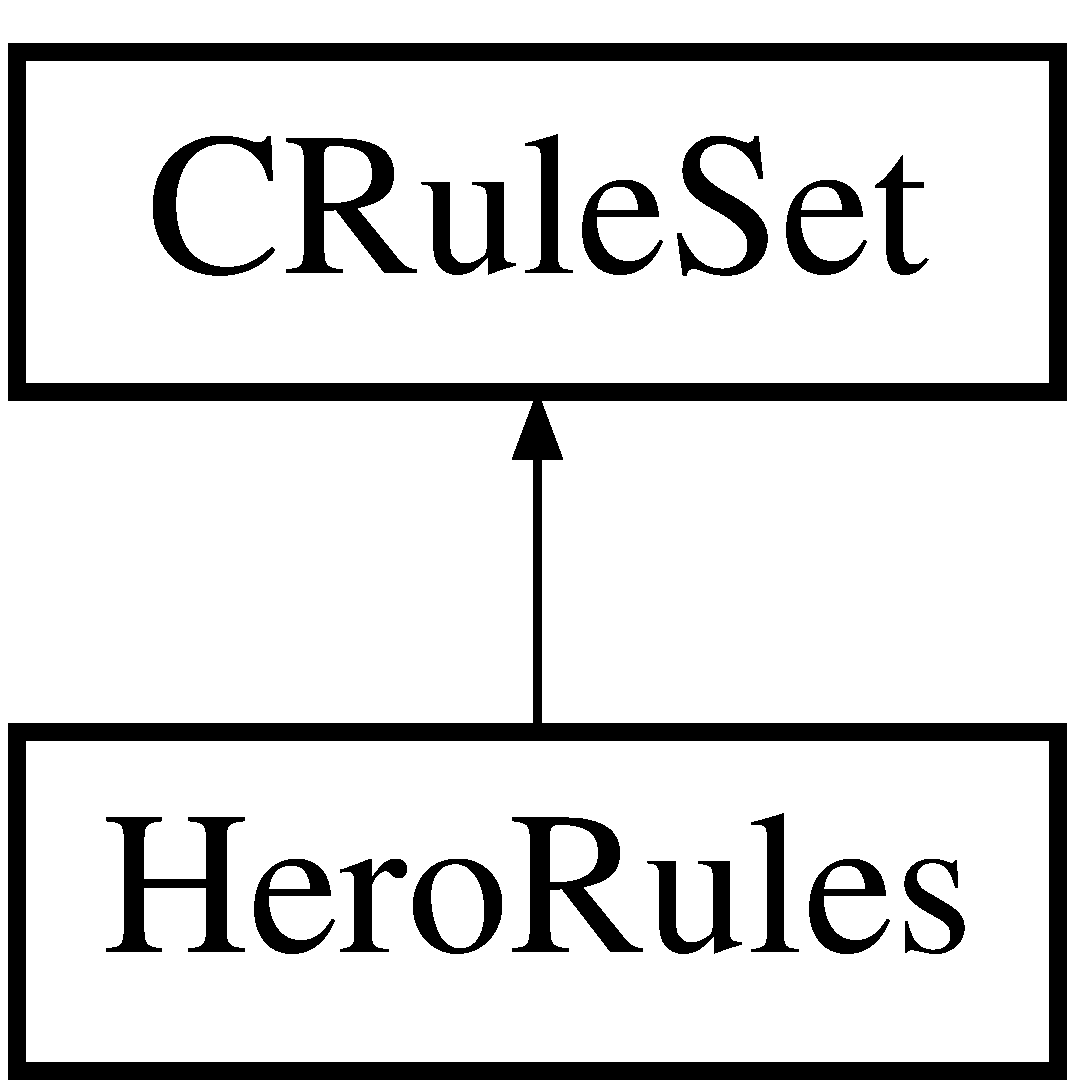
\includegraphics[height=2.000000cm]{class_hero_rules}
\end{center}
\end{figure}
\subsection*{Public Member Functions}
\begin{DoxyCompactItemize}
\item 
\mbox{\Hypertarget{class_hero_rules_a93fc8af4e87266175944bc917e5f3c42}\label{class_hero_rules_a93fc8af4e87266175944bc917e5f3c42}} 
{\bfseries Hero\+Rules} (\hyperlink{classmfg_1_1_engine}{mfg\+::\+Engine} $\ast$ge)
\item 
\mbox{\Hypertarget{class_hero_rules_a5e9001ef72079bf30525398c95acbd6e}\label{class_hero_rules_a5e9001ef72079bf30525398c95acbd6e}} 
virtual void {\bfseries apply} (\hyperlink{class_actor}{Actor} $\ast$)
\end{DoxyCompactItemize}
\subsection*{Additional Inherited Members}


\subsection{Detailed Description}
The \hyperlink{class_hero_rules}{Hero\+Rules} class -\/ define rules for a Hero \hyperlink{class_actor}{Actor}. 

The documentation for this class was generated from the following files\+:\begin{DoxyCompactItemize}
\item 
herorules.\+h\item 
herorules.\+cpp\end{DoxyCompactItemize}

\hypertarget{class_key_press_consumer}{}\section{Key\+Press\+Consumer Class Reference}
\label{class_key_press_consumer}\index{Key\+Press\+Consumer@{Key\+Press\+Consumer}}


The \hyperlink{class_key_press_consumer}{Key\+Press\+Consumer} class -\/ traps keyboard events so arrow keys can be filtered from application.  




{\ttfamily \#include $<$keypressconsumer.\+h$>$}

Inheritance diagram for Key\+Press\+Consumer\+:\begin{figure}[H]
\begin{center}
\leavevmode
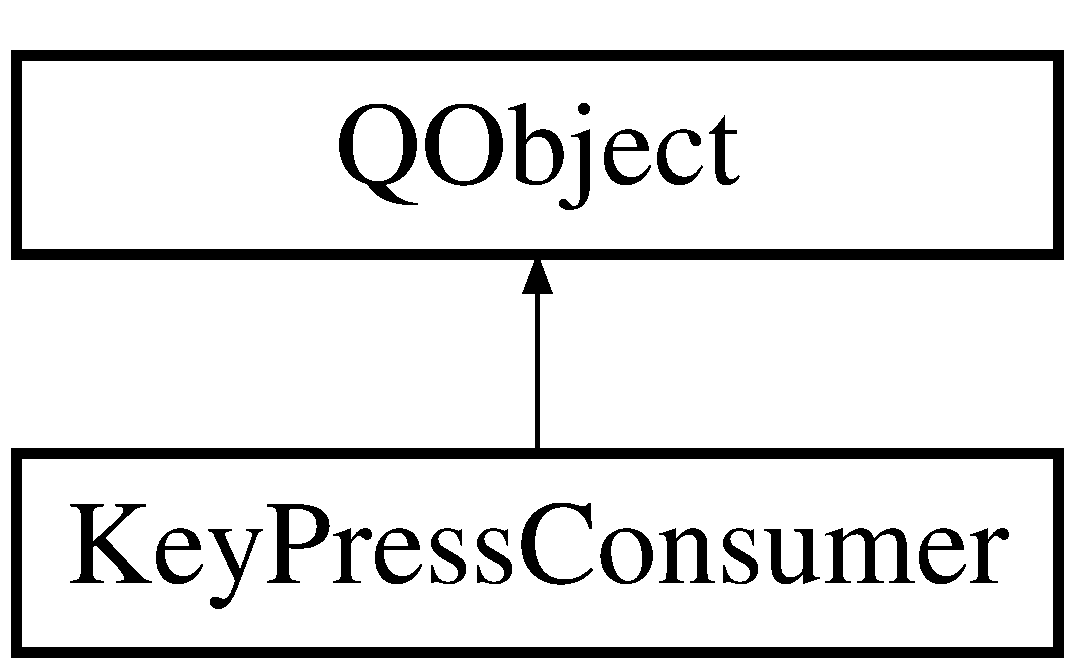
\includegraphics[height=2.000000cm]{class_key_press_consumer}
\end{center}
\end{figure}
\subsection*{Signals}
\begin{DoxyCompactItemize}
\item 
\mbox{\Hypertarget{class_key_press_consumer_aba09e00816c6024836487d2cb6249cd8}\label{class_key_press_consumer_aba09e00816c6024836487d2cb6249cd8}} 
void {\bfseries arrow\+Key} (Q\+Key\+Event $\ast$)
\end{DoxyCompactItemize}
\subsection*{Public Member Functions}
\begin{DoxyCompactItemize}
\item 
\mbox{\Hypertarget{class_key_press_consumer_a6f51041d96314790d033bce351b8f020}\label{class_key_press_consumer_a6f51041d96314790d033bce351b8f020}} 
{\bfseries Key\+Press\+Consumer} (Q\+Object $\ast$target, Q\+Object $\ast$parent=0)
\item 
\mbox{\Hypertarget{class_key_press_consumer_a2cbcc1db29e0447999a58f658cbae742}\label{class_key_press_consumer_a2cbcc1db29e0447999a58f658cbae742}} 
Q\+Object $\ast$ {\bfseries target} () const
\item 
\mbox{\Hypertarget{class_key_press_consumer_abcbcaf5a0c8e1d04b134e6b65b53ad7e}\label{class_key_press_consumer_abcbcaf5a0c8e1d04b134e6b65b53ad7e}} 
void {\bfseries set\+Target} (Q\+Object $\ast$target)
\end{DoxyCompactItemize}
\subsection*{Protected Member Functions}
\begin{DoxyCompactItemize}
\item 
\mbox{\Hypertarget{class_key_press_consumer_a375adc3bbaababb0e7a6aee2e12d99c6}\label{class_key_press_consumer_a375adc3bbaababb0e7a6aee2e12d99c6}} 
bool {\bfseries event\+Filter} (Q\+Object $\ast$obj, Q\+Event $\ast$event)
\end{DoxyCompactItemize}
\subsection*{Private Attributes}
\begin{DoxyCompactItemize}
\item 
\mbox{\Hypertarget{class_key_press_consumer_a4270d30101dac8588fa1603ce3f573c6}\label{class_key_press_consumer_a4270d30101dac8588fa1603ce3f573c6}} 
Q\+Object $\ast$ {\bfseries m\+\_\+target}
\end{DoxyCompactItemize}


\subsection{Detailed Description}
The \hyperlink{class_key_press_consumer}{Key\+Press\+Consumer} class -\/ traps keyboard events so arrow keys can be filtered from application. 

The documentation for this class was generated from the following files\+:\begin{DoxyCompactItemize}
\item 
keypressconsumer.\+h\item 
keypressconsumer.\+cpp\end{DoxyCompactItemize}

\hypertarget{class_main_window}{}\section{Main\+Window Class Reference}
\label{class_main_window}\index{Main\+Window@{Main\+Window}}


The \hyperlink{class_main_window}{Main\+Window} class -\/ Defines Main window for application.  




{\ttfamily \#include $<$mainwindow.\+h$>$}

Inheritance diagram for Main\+Window\+:\begin{figure}[H]
\begin{center}
\leavevmode
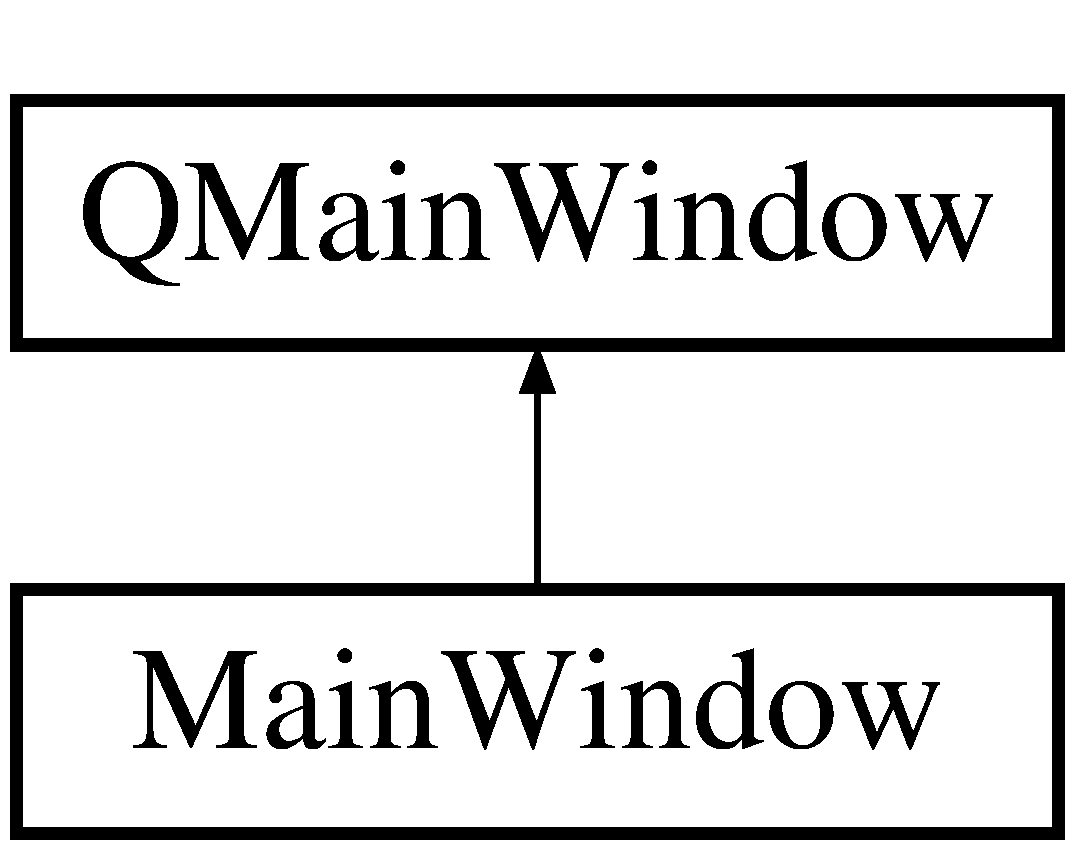
\includegraphics[height=2.000000cm]{class_main_window}
\end{center}
\end{figure}
\subsection*{Public Slots}
\begin{DoxyCompactItemize}
\item 
\mbox{\Hypertarget{class_main_window_ae2183a75f745a295c966f07aba433a3d}\label{class_main_window_ae2183a75f745a295c966f07aba433a3d}} 
void {\bfseries add\+Male\+Villager} ()
\item 
\mbox{\Hypertarget{class_main_window_a7ae250e3b7f9e69b32228d22ea27aea6}\label{class_main_window_a7ae250e3b7f9e69b32228d22ea27aea6}} 
void {\bfseries add\+Female\+Villager} ()
\item 
\mbox{\Hypertarget{class_main_window_a543edb288ac3215527861c7b12cedf6a}\label{class_main_window_a543edb288ac3215527861c7b12cedf6a}} 
void {\bfseries add\+Hero} ()
\item 
\mbox{\Hypertarget{class_main_window_a50b51e610d079d24de857dd0bbf9e209}\label{class_main_window_a50b51e610d079d24de857dd0bbf9e209}} 
void {\bfseries add\+Monster} ()
\item 
\mbox{\Hypertarget{class_main_window_aafdc6845a18fbc27e50e4e5b1a0b46f5}\label{class_main_window_aafdc6845a18fbc27e50e4e5b1a0b46f5}} 
void {\bfseries add\+Scheusal} ()
\item 
\mbox{\Hypertarget{class_main_window_a4ee53a86fe9a84b09d46bb99278c8bc1}\label{class_main_window_a4ee53a86fe9a84b09d46bb99278c8bc1}} 
void {\bfseries add\+Mountain} ()
\item 
\mbox{\Hypertarget{class_main_window_a853add69be543fb60126fd04d90cb278}\label{class_main_window_a853add69be543fb60126fd04d90cb278}} 
void {\bfseries show\+Console} ()
\item 
\mbox{\Hypertarget{class_main_window_a6834d440788437b3c276be1e697f2c0a}\label{class_main_window_a6834d440788437b3c276be1e697f2c0a}} 
void {\bfseries add\+Stream} ()
\item 
\mbox{\Hypertarget{class_main_window_a1338e470b7a7a8715c032c0e859196b2}\label{class_main_window_a1338e470b7a7a8715c032c0e859196b2}} 
void {\bfseries console\+Text} (const char $\ast$)
\item 
\mbox{\Hypertarget{class_main_window_a1b5e18cb44047a2b1bd937541b3703fc}\label{class_main_window_a1b5e18cb44047a2b1bd937541b3703fc}} 
void {\bfseries sprite\+Down} ()
\item 
\mbox{\Hypertarget{class_main_window_a7e31e60d4f2c0263e42ce22a08b1b660}\label{class_main_window_a7e31e60d4f2c0263e42ce22a08b1b660}} 
void {\bfseries sprite\+Left} ()
\item 
\mbox{\Hypertarget{class_main_window_a68db96473e3609664bd2c4a5a9afd5ee}\label{class_main_window_a68db96473e3609664bd2c4a5a9afd5ee}} 
void {\bfseries sprite\+Right} ()
\item 
\mbox{\Hypertarget{class_main_window_a724d1d00a423a663cd218ccb8de6125f}\label{class_main_window_a724d1d00a423a663cd218ccb8de6125f}} 
void {\bfseries sprite\+Speed\+Fast} ()
\item 
\mbox{\Hypertarget{class_main_window_a4e06a1b132302f5cbb384c69706bf177}\label{class_main_window_a4e06a1b132302f5cbb384c69706bf177}} 
void {\bfseries sprite\+Speed\+Slow} ()
\item 
\mbox{\Hypertarget{class_main_window_a4019b442b2b22a62285f5bb362e10fa4}\label{class_main_window_a4019b442b2b22a62285f5bb362e10fa4}} 
void {\bfseries sprite\+Up} ()
\item 
\mbox{\Hypertarget{class_main_window_a9054e450ac01e29b3394e3dea19dcb9f}\label{class_main_window_a9054e450ac01e29b3394e3dea19dcb9f}} 
void {\bfseries sprite\+Stop} ()
\item 
\mbox{\Hypertarget{class_main_window_a2a5c09d44d9953048f8f753bee4442d2}\label{class_main_window_a2a5c09d44d9953048f8f753bee4442d2}} 
void {\bfseries sprite\+Start} ()
\item 
\mbox{\Hypertarget{class_main_window_aacd1780f177b9ca508d68586b76b76cd}\label{class_main_window_aacd1780f177b9ca508d68586b76b76cd}} 
void {\bfseries stop\+Scene} ()
\item 
\mbox{\Hypertarget{class_main_window_a663daceb7fc6dade28996c0037cbce02}\label{class_main_window_a663daceb7fc6dade28996c0037cbce02}} 
void {\bfseries start\+Scene} ()
\item 
\mbox{\Hypertarget{class_main_window_aadcf009c25064b97b2b76895ccc4150a}\label{class_main_window_aadcf009c25064b97b2b76895ccc4150a}} 
void {\bfseries update\+Game\+Status} ()
\item 
\mbox{\Hypertarget{class_main_window_acf42224e60d71ebd981eb36b51c31eec}\label{class_main_window_acf42224e60d71ebd981eb36b51c31eec}} 
void {\bfseries spawn\+All} ()
\item 
\mbox{\Hypertarget{class_main_window_ad1a991e51cf88dd4c5471256e5d84bd9}\label{class_main_window_ad1a991e51cf88dd4c5471256e5d84bd9}} 
void {\bfseries clear\+Actors} ()
\item 
\mbox{\Hypertarget{class_main_window_acbb51ed12285e43995e2795c0a8b847b}\label{class_main_window_acbb51ed12285e43995e2795c0a8b847b}} 
void {\bfseries music\+On} ()
\item 
\mbox{\Hypertarget{class_main_window_a00caa93f8f96a6b5b1d6c991afc090b6}\label{class_main_window_a00caa93f8f96a6b5b1d6c991afc090b6}} 
void {\bfseries music\+Off} ()
\item 
\mbox{\Hypertarget{class_main_window_a7eada83031022060e247636a27d4b6fc}\label{class_main_window_a7eada83031022060e247636a27d4b6fc}} 
void {\bfseries change\+Volume} (int)
\item 
\mbox{\Hypertarget{class_main_window_a09fe9270f0534ecf9e7acea4d1eaf8c4}\label{class_main_window_a09fe9270f0534ecf9e7acea4d1eaf8c4}} 
void {\bfseries actor\+Clicked} (Q\+Graphics\+Scene\+Mouse\+Event $\ast$, \hyperlink{class_sprite}{Sprite} $\ast$)
\item 
\mbox{\Hypertarget{class_main_window_adf88315e557e377353059bd313b1bfa6}\label{class_main_window_adf88315e557e377353059bd313b1bfa6}} 
void {\bfseries key\+Press\+Event} (Q\+Key\+Event $\ast$e)
\item 
\mbox{\Hypertarget{class_main_window_a04b0c8ff3be04d1b1bf54e78c5ee7039}\label{class_main_window_a04b0c8ff3be04d1b1bf54e78c5ee7039}} 
void {\bfseries key\+Release\+Event} (Q\+Key\+Event $\ast$e)
\item 
\mbox{\Hypertarget{class_main_window_afded6dc0db0f820485fda0ea61675e7c}\label{class_main_window_afded6dc0db0f820485fda0ea61675e7c}} 
void {\bfseries scale\+Scene} (int s)
\end{DoxyCompactItemize}
\subsection*{Public Member Functions}
\begin{DoxyCompactItemize}
\item 
\mbox{\Hypertarget{class_main_window_a8b244be8b7b7db1b08de2a2acb9409db}\label{class_main_window_a8b244be8b7b7db1b08de2a2acb9409db}} 
{\bfseries Main\+Window} (Q\+Widget $\ast$parent=0)
\item 
\mbox{\Hypertarget{class_main_window_a8876be87b41337f2ccf8ef1fc6b4a9c8}\label{class_main_window_a8876be87b41337f2ccf8ef1fc6b4a9c8}} 
\hyperlink{class_game_scene}{Game\+Scene} $\ast$ {\bfseries scene} ()
\item 
\mbox{\Hypertarget{class_main_window_a0eae38634f26f1bd23717174cd751523}\label{class_main_window_a0eae38634f26f1bd23717174cd751523}} 
void {\bfseries scene} (\hyperlink{class_game_scene}{Game\+Scene} $\ast$)
\item 
\mbox{\Hypertarget{class_main_window_ae9adbd9ad74d836628ff2950d503e397}\label{class_main_window_ae9adbd9ad74d836628ff2950d503e397}} 
Q\+Timer $\ast$ {\bfseries timer} ()
\item 
\mbox{\Hypertarget{class_main_window_a5ac9feeab611a5aafaa0191df82b4bf1}\label{class_main_window_a5ac9feeab611a5aafaa0191df82b4bf1}} 
void {\bfseries timer} (Q\+Timer $\ast$)
\item 
\mbox{\Hypertarget{class_main_window_a1ee03f14689d63b79b48dd31c7f2c572}\label{class_main_window_a1ee03f14689d63b79b48dd31c7f2c572}} 
Q\+Media\+Player $\ast$ {\bfseries media\+Player} () const
\item 
\mbox{\Hypertarget{class_main_window_a04a7066651d54008b870b722b310da41}\label{class_main_window_a04a7066651d54008b870b722b310da41}} 
void {\bfseries media\+Player} (Q\+Media\+Player $\ast$media\+Player)
\item 
\mbox{\Hypertarget{class_main_window_adb747cc217a5a2a077af79fe72c278cf}\label{class_main_window_adb747cc217a5a2a077af79fe72c278cf}} 
Q\+Label $\ast$ {\bfseries status\+\_\+label} () const
\item 
\mbox{\Hypertarget{class_main_window_a685d2e26a50d151d9ebd4fb0cc9f8aca}\label{class_main_window_a685d2e26a50d151d9ebd4fb0cc9f8aca}} 
void {\bfseries status\+\_\+label} (Q\+Label $\ast$status\+\_\+label)
\item 
\mbox{\Hypertarget{class_main_window_a5f010205227b4aaf83f3874d5fbb08a0}\label{class_main_window_a5f010205227b4aaf83f3874d5fbb08a0}} 
\hyperlink{class_console_widget}{Console\+Widget} $\ast$ {\bfseries console} () const
\item 
\mbox{\Hypertarget{class_main_window_a1fabca5cc1f1f4f6a4a1cecec17aa822}\label{class_main_window_a1fabca5cc1f1f4f6a4a1cecec17aa822}} 
void {\bfseries show\+Scene} (const Q\+String \&name)
\end{DoxyCompactItemize}
\subsection*{Protected Slots}
\begin{DoxyCompactItemize}
\item 
\mbox{\Hypertarget{class_main_window_a34e60652ff3e3db88a02ed27dd1b65f6}\label{class_main_window_a34e60652ff3e3db88a02ed27dd1b65f6}} 
void {\bfseries update\+Sprite\+Position} (\hyperlink{class_sprite}{Sprite} $\ast$sprite)
\end{DoxyCompactItemize}
\subsection*{Protected Member Functions}
\begin{DoxyCompactItemize}
\item 
\mbox{\Hypertarget{class_main_window_abad7b29bc1e42b37a722bf063aab3512}\label{class_main_window_abad7b29bc1e42b37a722bf063aab3512}} 
\hyperlink{class_actor}{Scene\+Actor} $\ast$ {\bfseries add\+Actor} (const Q\+String \&name)
\item 
\mbox{\Hypertarget{class_main_window_a15a2912e758dcab1067e058c05f0985c}\label{class_main_window_a15a2912e758dcab1067e058c05f0985c}} 
\hyperlink{class_sprite}{Sprite} $\ast$ {\bfseries current\+Sprite} () const
\item 
\mbox{\Hypertarget{class_main_window_aa8933698bfe5ca463cb69879663b573a}\label{class_main_window_aa8933698bfe5ca463cb69879663b573a}} 
void {\bfseries current\+Sprite} (\hyperlink{class_sprite}{Sprite} $\ast$current\+Sprite)
\end{DoxyCompactItemize}
\subsection*{Private Member Functions}
\begin{DoxyCompactItemize}
\item 
\mbox{\Hypertarget{class_main_window_ad241698f69fdcf66d792f8ce6064a154}\label{class_main_window_ad241698f69fdcf66d792f8ce6064a154}} 
void {\bfseries move\+Sprite} (Sprite\+\_\+\+Direction)
\item 
\mbox{\Hypertarget{class_main_window_ad3776dfddc6ea10ce6331f1c142ac1ac}\label{class_main_window_ad3776dfddc6ea10ce6331f1c142ac1ac}} 
void {\bfseries setup\+Timer} ()
\item 
\mbox{\Hypertarget{class_main_window_a56ac2c93f1c691df939808c909140eb1}\label{class_main_window_a56ac2c93f1c691df939808c909140eb1}} 
void {\bfseries show\+Melba} ()
\item 
\mbox{\Hypertarget{class_main_window_acf0d2ef2d17eb4b58e77b24574a244fd}\label{class_main_window_acf0d2ef2d17eb4b58e77b24574a244fd}} 
void {\bfseries show\+Space} ()
\item 
\mbox{\Hypertarget{class_main_window_a354de8b79b7996530d6689c1a68cf858}\label{class_main_window_a354de8b79b7996530d6689c1a68cf858}} 
void {\bfseries setup\+Status\+Label} ()
\item 
\mbox{\Hypertarget{class_main_window_aa4907b0251d305659e403c62921ef331}\label{class_main_window_aa4907b0251d305659e403c62921ef331}} 
void \hyperlink{class_main_window_aa4907b0251d305659e403c62921ef331}{create\+Menus} ()
\begin{DoxyCompactList}\small\item\em \hyperlink{class_main_window_aa4907b0251d305659e403c62921ef331}{Main\+Window\+::create\+Menus}. \end{DoxyCompactList}\item 
Q\+Action $\ast$ \hyperlink{class_main_window_a5916e4c4ce07f6de5e084d0cd27d81c2}{create\+Action} (const Q\+String \&menu, const Q\+Key\+Sequence \&, const Q\+String \&tip)
\begin{DoxyCompactList}\small\item\em \hyperlink{class_main_window_a5916e4c4ce07f6de5e084d0cd27d81c2}{Main\+Window\+::create\+Action} create a menu action. \end{DoxyCompactList}\item 
\mbox{\Hypertarget{class_main_window_a69f73b93cc05c89a9ae1be0161105982}\label{class_main_window_a69f73b93cc05c89a9ae1be0161105982}} 
void \hyperlink{class_main_window_a69f73b93cc05c89a9ae1be0161105982}{new\+File} ()
\begin{DoxyCompactList}\small\item\em \hyperlink{class_main_window_a69f73b93cc05c89a9ae1be0161105982}{Main\+Window\+::new\+File} -- T\+O\+DO. \end{DoxyCompactList}\item 
\mbox{\Hypertarget{class_main_window_a288b768c3c21a9171bdc56fe845ece8b}\label{class_main_window_a288b768c3c21a9171bdc56fe845ece8b}} 
void {\bfseries open\+File} ()
\item 
\mbox{\Hypertarget{class_main_window_a464aaa4d378e7b2d814756a73d6e1ed6}\label{class_main_window_a464aaa4d378e7b2d814756a73d6e1ed6}} 
void {\bfseries save\+File} ()
\end{DoxyCompactItemize}
\subsection*{Private Attributes}
\begin{DoxyCompactItemize}
\item 
\mbox{\Hypertarget{class_main_window_aae99b6542b0f957e696d7b41bbabb4c5}\label{class_main_window_aae99b6542b0f957e696d7b41bbabb4c5}} 
\hyperlink{class_game_scene}{Game\+Scene} $\ast$ {\bfseries m\+\_\+scene}
\item 
\mbox{\Hypertarget{class_main_window_af518103f9ff2412885727105adc7e165}\label{class_main_window_af518103f9ff2412885727105adc7e165}} 
Q\+Graphics\+Rect\+Item $\ast$ {\bfseries rectangle}
\item 
\mbox{\Hypertarget{class_main_window_af74cc34242d09f3b3c4590c7505ada4e}\label{class_main_window_af74cc34242d09f3b3c4590c7505ada4e}} 
Q\+Graphics\+Ellipse\+Item $\ast$ {\bfseries ellipse}
\item 
\mbox{\Hypertarget{class_main_window_a467644eafb91dadf1458b6fac3cab704}\label{class_main_window_a467644eafb91dadf1458b6fac3cab704}} 
Q\+Graphics\+Text\+Item $\ast$ {\bfseries text}
\item 
\mbox{\Hypertarget{class_main_window_a0ccba9e29a838a159b08a6ffa9556103}\label{class_main_window_a0ccba9e29a838a159b08a6ffa9556103}} 
\hyperlink{class_sprite}{Sprite} $\ast$ {\bfseries m\+\_\+current\+\_\+sprite}
\item 
\mbox{\Hypertarget{class_main_window_a9628f6c87ca0ec54ca4f53a00d8abdbe}\label{class_main_window_a9628f6c87ca0ec54ca4f53a00d8abdbe}} 
Q\+Label $\ast$ {\bfseries m\+\_\+status\+\_\+label}
\item 
\mbox{\Hypertarget{class_main_window_a7efd59ad07ae26f00d1da33615a46f0c}\label{class_main_window_a7efd59ad07ae26f00d1da33615a46f0c}} 
Q\+Timer $\ast$ {\bfseries m\+\_\+timer}
\item 
\mbox{\Hypertarget{class_main_window_ab4d7b03ca7aee1f7b2f3556d408048bd}\label{class_main_window_ab4d7b03ca7aee1f7b2f3556d408048bd}} 
Q\+Media\+Player $\ast$ {\bfseries m\+\_\+player}
\item 
\mbox{\Hypertarget{class_main_window_aa3e10b46a96bb420449980caeadeb79f}\label{class_main_window_aa3e10b46a96bb420449980caeadeb79f}} 
Key\+State {\bfseries m\+\_\+key\+\_\+state}
\item 
\mbox{\Hypertarget{class_main_window_a55e40849a54cbfed1c557dd3cb798d9c}\label{class_main_window_a55e40849a54cbfed1c557dd3cb798d9c}} 
\hyperlink{class_console_widget}{Console\+Widget} $\ast$ {\bfseries m\+\_\+console}
\item 
\mbox{\Hypertarget{class_main_window_a35466a70ed47252a0191168126a352a5}\label{class_main_window_a35466a70ed47252a0191168126a352a5}} 
Ui\+::\+Main\+Window $\ast$ {\bfseries ui}
\end{DoxyCompactItemize}


\subsection{Detailed Description}
The \hyperlink{class_main_window}{Main\+Window} class -\/ Defines Main window for application. 

\subsection{Member Function Documentation}
\mbox{\Hypertarget{class_main_window_a5916e4c4ce07f6de5e084d0cd27d81c2}\label{class_main_window_a5916e4c4ce07f6de5e084d0cd27d81c2}} 
\index{Main\+Window@{Main\+Window}!create\+Action@{create\+Action}}
\index{create\+Action@{create\+Action}!Main\+Window@{Main\+Window}}
\subsubsection{\texorpdfstring{create\+Action()}{createAction()}}
{\footnotesize\ttfamily Q\+Action $\ast$ Main\+Window\+::create\+Action (\begin{DoxyParamCaption}\item[{const Q\+String \&}]{menu,  }\item[{const Q\+Key\+Sequence \&}]{shortcut,  }\item[{const Q\+String \&}]{tip }\end{DoxyParamCaption})\hspace{0.3cm}{\ttfamily [private]}}



\hyperlink{class_main_window_a5916e4c4ce07f6de5e084d0cd27d81c2}{Main\+Window\+::create\+Action} create a menu action. 


\begin{DoxyParams}{Parameters}
{\em menu} & \\
\hline
{\em shortcut} & \\
\hline
{\em tip} & \\
\hline
\end{DoxyParams}
\begin{DoxyReturn}{Returns}
$\ast$\+Q\+Action 
\end{DoxyReturn}

\begin{DoxyCode}
137                                                                                                       \{
138     QAction *newAct = \textcolor{keyword}{new} QAction(tr(menu.toLatin1().data()), \textcolor{keyword}{this});
139     newAct->setShortcut(shortcut);
140     newAct->setStatusTip(tr(tip.toLatin1().data()));
141     \textcolor{keywordflow}{return} newAct;
142 \}
\end{DoxyCode}


The documentation for this class was generated from the following files\+:\begin{DoxyCompactItemize}
\item 
mainwindow.\+h\item 
mainwindow.\+cpp\end{DoxyCompactItemize}

\hypertarget{class_monster_rules}{}\section{Monster\+Rules Class Reference}
\label{class_monster_rules}\index{Monster\+Rules@{Monster\+Rules}}
Inheritance diagram for Monster\+Rules\+:\begin{figure}[H]
\begin{center}
\leavevmode
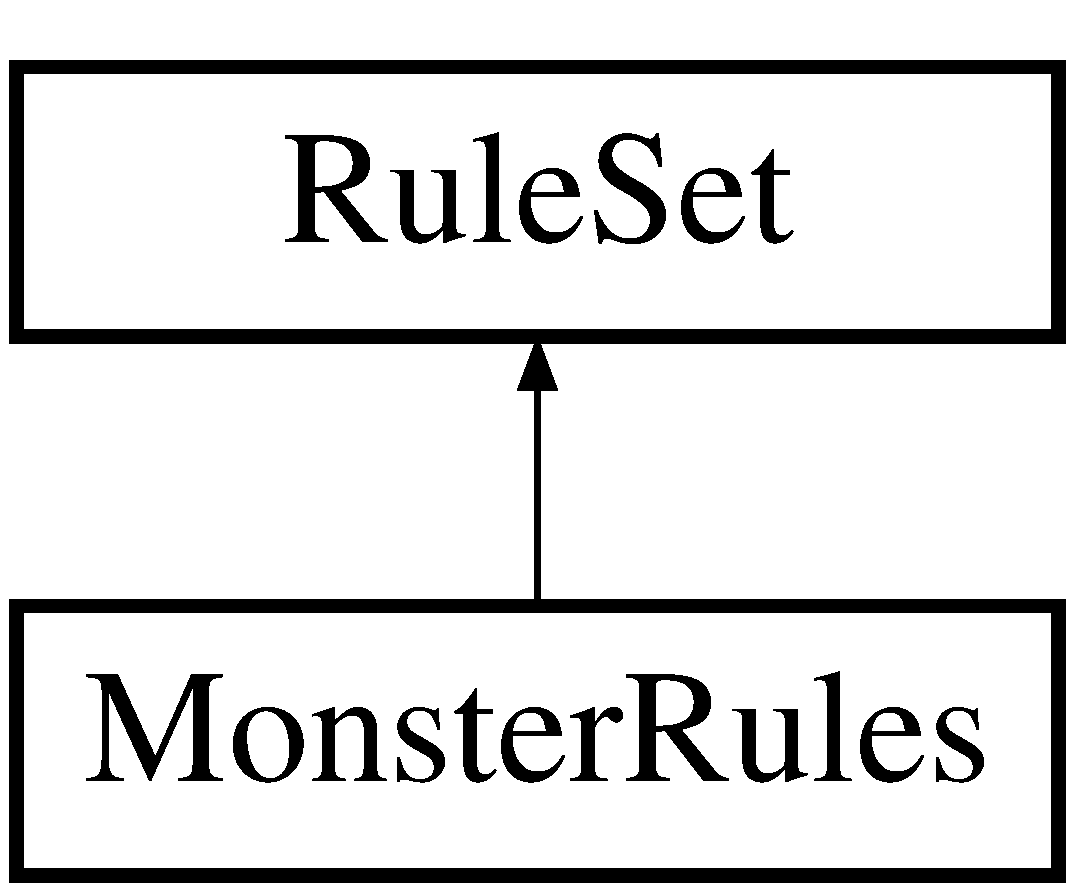
\includegraphics[height=2.000000cm]{class_monster_rules}
\end{center}
\end{figure}
\subsection*{Public Member Functions}
\begin{DoxyCompactItemize}
\item 
\mbox{\Hypertarget{class_monster_rules_a054cd4fe8f7aef6b17e5338c7d298582}\label{class_monster_rules_a054cd4fe8f7aef6b17e5338c7d298582}} 
{\bfseries Monster\+Rules} (\hyperlink{classmfg_1_1_engine}{mfg\+::\+Engine} $\ast$ge)
\item 
\mbox{\Hypertarget{class_monster_rules_afeaa7b20a44ec650f48e53a81639d7b4}\label{class_monster_rules_afeaa7b20a44ec650f48e53a81639d7b4}} 
virtual void {\bfseries apply} (\hyperlink{class_actor}{Actor} $\ast$)
\end{DoxyCompactItemize}
\subsection*{Additional Inherited Members}


The documentation for this class was generated from the following files\+:\begin{DoxyCompactItemize}
\item 
monsterrules.\+h\item 
monsterrules.\+cpp\end{DoxyCompactItemize}

\hypertarget{class_rule_set}{}\section{Rule\+Set Class Reference}
\label{class_rule_set}\index{Rule\+Set@{Rule\+Set}}


The \hyperlink{class_rule_set}{Rule\+Set} class -\/ define rules for characters.  




{\ttfamily \#include $<$ruleset.\+h$>$}

Inheritance diagram for Rule\+Set\+:\begin{figure}[H]
\begin{center}
\leavevmode
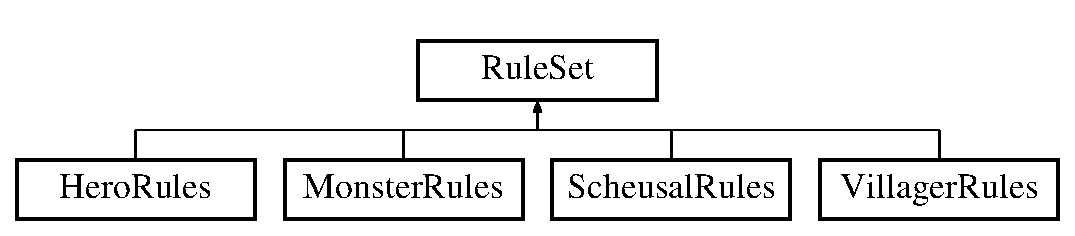
\includegraphics[height=2.000000cm]{class_rule_set}
\end{center}
\end{figure}
\subsection*{Public Member Functions}
\begin{DoxyCompactItemize}
\item 
\mbox{\Hypertarget{class_rule_set_af7f8610fe8222f6f72a3c1745fa53548}\label{class_rule_set_af7f8610fe8222f6f72a3c1745fa53548}} 
{\bfseries Rule\+Set} (\hyperlink{classmfg_1_1_engine}{mfg\+::\+Engine} $\ast$ge)
\item 
\mbox{\Hypertarget{class_rule_set_a9666dd442a664846c558a10403f22a89}\label{class_rule_set_a9666dd442a664846c558a10403f22a89}} 
virtual void {\bfseries apply} (\hyperlink{class_actor}{Actor} $\ast$)=0
\item 
\mbox{\Hypertarget{class_rule_set_a48232bc120a79ee41ab79b63a3825b37}\label{class_rule_set_a48232bc120a79ee41ab79b63a3825b37}} 
\hyperlink{class_actor}{Actor} $\ast$ {\bfseries actor} (\hyperlink{class_actor}{Actor} $\ast$actor)
\item 
\mbox{\Hypertarget{class_rule_set_ac1c666adae22de45e62636ba423cc60c}\label{class_rule_set_ac1c666adae22de45e62636ba423cc60c}} 
\hyperlink{class_actor}{Actor} $\ast$ {\bfseries actor} ()
\item 
\mbox{\Hypertarget{class_rule_set_aecfc0deb351d3a86c2a2a4321bb7002c}\label{class_rule_set_aecfc0deb351d3a86c2a2a4321bb7002c}} 
Q\+Json\+Array {\bfseries friends} ()
\item 
\mbox{\Hypertarget{class_rule_set_abc260d8a6e24ad6f075f1360f94760d5}\label{class_rule_set_abc260d8a6e24ad6f075f1360f94760d5}} 
Q\+Json\+Array {\bfseries foes} ()
\end{DoxyCompactItemize}
\subsection*{Protected Attributes}
\begin{DoxyCompactItemize}
\item 
\mbox{\Hypertarget{class_rule_set_ad6f6ce80af76542f89bc4a9557708b4a}\label{class_rule_set_ad6f6ce80af76542f89bc4a9557708b4a}} 
Q\+Json\+Array {\bfseries m\+\_\+friends}
\item 
\mbox{\Hypertarget{class_rule_set_a604539c01fc13d94ee8242e484d21a50}\label{class_rule_set_a604539c01fc13d94ee8242e484d21a50}} 
Q\+Json\+Array {\bfseries m\+\_\+foes}
\item 
\mbox{\Hypertarget{class_rule_set_adeb1310cc1a39af21ca3ce37f99e332e}\label{class_rule_set_adeb1310cc1a39af21ca3ce37f99e332e}} 
\hyperlink{classmfg_1_1_engine}{mfg\+::\+Engine} $\ast$ {\bfseries m\+\_\+game\+\_\+engine}
\end{DoxyCompactItemize}
\subsection*{Private Attributes}
\begin{DoxyCompactItemize}
\item 
\mbox{\Hypertarget{class_rule_set_ae91eb402b95d7fc606fa514b2feec0ce}\label{class_rule_set_ae91eb402b95d7fc606fa514b2feec0ce}} 
\hyperlink{class_actor}{Actor} $\ast$ {\bfseries m\+\_\+actor}
\end{DoxyCompactItemize}


\subsection{Detailed Description}
The \hyperlink{class_rule_set}{Rule\+Set} class -\/ define rules for characters. 

The documentation for this class was generated from the following files\+:\begin{DoxyCompactItemize}
\item 
ruleset.\+h\item 
ruleset.\+cpp\end{DoxyCompactItemize}

\hypertarget{class_scene_manager}{}\section{Scene\+Manager Class Reference}
\label{class_scene_manager}\index{Scene\+Manager@{Scene\+Manager}}


The \hyperlink{class_scene_manager}{Scene\+Manager} class -\/ defines a \hyperlink{class_scene_manager}{Scene\+Manager}.  




{\ttfamily \#include $<$scenemanager.\+h$>$}

\subsection*{Public Member Functions}
\begin{DoxyCompactItemize}
\item 
\mbox{\Hypertarget{class_scene_manager_a017968ad7fea883b37597ccd43ee8d21}\label{class_scene_manager_a017968ad7fea883b37597ccd43ee8d21}} 
{\bfseries Scene\+Manager} (\hyperlink{classmfg_1_1_engine}{mfg\+::\+Engine} $\ast$engine)
\item 
\hyperlink{class_game_scene}{Game\+Scene} $\ast$ \hyperlink{class_scene_manager_ac862660ed44b8ab110dec97ec90a9bad}{create\+Scene} (const Q\+String \&name, C\+Object $\ast$parent)
\begin{DoxyCompactList}\small\item\em \hyperlink{class_scene_manager_ac862660ed44b8ab110dec97ec90a9bad}{Scene\+Manager\+::create\+Scene} creates the scene by name T\+O\+DO\+: build scene from json description if available. \end{DoxyCompactList}\item 
\mbox{\Hypertarget{class_scene_manager_a1f8394061bc73982c2893bb4984f4542}\label{class_scene_manager_a1f8394061bc73982c2893bb4984f4542}} 
\hyperlink{class_game_scene}{Game\+Scene} $\ast$ {\bfseries get\+Scene} (const Q\+String \&name)
\item 
\mbox{\Hypertarget{class_scene_manager_a249162f1c24a0960e354a67cf9ed039d}\label{class_scene_manager_a249162f1c24a0960e354a67cf9ed039d}} 
\hyperlink{classmfg_1_1_engine}{mfg\+::\+Engine} $\ast$ {\bfseries game\+\_\+engine} ()
\end{DoxyCompactItemize}
\subsection*{Private Attributes}
\begin{DoxyCompactItemize}
\item 
\mbox{\Hypertarget{class_scene_manager_a487426cfd98ef3b57a7b0192d490b4ae}\label{class_scene_manager_a487426cfd98ef3b57a7b0192d490b4ae}} 
\hyperlink{classmfg_1_1_engine}{mfg\+::\+Engine} $\ast$ {\bfseries m\+\_\+engine}
\item 
\mbox{\Hypertarget{class_scene_manager_a84a59de256b2d0c2574d77c62b0f4ff3}\label{class_scene_manager_a84a59de256b2d0c2574d77c62b0f4ff3}} 
Scene\+Map {\bfseries m\+\_\+scene\+\_\+map}
\end{DoxyCompactItemize}


\subsection{Detailed Description}
The \hyperlink{class_scene_manager}{Scene\+Manager} class -\/ defines a \hyperlink{class_scene_manager}{Scene\+Manager}. 

\subsection{Member Function Documentation}
\mbox{\Hypertarget{class_scene_manager_ac862660ed44b8ab110dec97ec90a9bad}\label{class_scene_manager_ac862660ed44b8ab110dec97ec90a9bad}} 
\index{Scene\+Manager@{Scene\+Manager}!create\+Scene@{create\+Scene}}
\index{create\+Scene@{create\+Scene}!Scene\+Manager@{Scene\+Manager}}
\subsubsection{\texorpdfstring{create\+Scene()}{createScene()}}
{\footnotesize\ttfamily \hyperlink{class_game_scene}{Game\+Scene} $\ast$ Scene\+Manager\+::create\+Scene (\begin{DoxyParamCaption}\item[{const Q\+String \&}]{name,  }\item[{C\+Object $\ast$}]{parent }\end{DoxyParamCaption})}



\hyperlink{class_scene_manager_ac862660ed44b8ab110dec97ec90a9bad}{Scene\+Manager\+::create\+Scene} creates the scene by name T\+O\+DO\+: build scene from json description if available. 


\begin{DoxyParams}{Parameters}
{\em name\+:string} & the name of the scene \\
\hline
{\em parent} & the parent for the scene, usually the main window \\
\hline
\end{DoxyParams}
\begin{DoxyReturn}{Returns}
scene the newly created scene 
\end{DoxyReturn}

\begin{DoxyCode}
23                                                                         \{
24     QString settings;
25     QFile file;
26     file.setFileName(\textcolor{stringliteral}{":/config/scenes/"}+name+\textcolor{stringliteral}{".json"});
27     file.open(QIODevice::ReadOnly | QIODevice::Text);
28     settings = file.readAll();
29     file.close();
30     QJsonDocument sd = QJsonDocument::fromJson(settings.toUtf8());
31     \textcolor{keywordflow}{if}(sd.isEmpty()) \{
32         \textcolor{keywordflow}{throw} \textcolor{stringliteral}{"Error with JSON Document: "} + name + \textcolor{stringliteral}{".json"};
33     \}
34     QJsonObject sett2 = sd.object();
35     \textcolor{keyword}{auto} properties = sett2[\textcolor{stringliteral}{"properties"}].toObject();
36     \textcolor{keywordtype}{int} x = properties[\textcolor{stringliteral}{"rect"}].toObject()[\textcolor{stringliteral}{"x"}].toInt();
37     \textcolor{keywordtype}{int} y = properties[\textcolor{stringliteral}{"rect"}].toObject()[\textcolor{stringliteral}{"y"}].toInt();
38     \textcolor{keywordtype}{int} width = properties[\textcolor{stringliteral}{"rect"}].toObject()[\textcolor{stringliteral}{"width"}].toInt();
39     \textcolor{keywordtype}{int} height = properties[\textcolor{stringliteral}{"rect"}].toObject()[\textcolor{stringliteral}{"height"}].toInt();
40     \hyperlink{class_game_scene}{GameScene} *scene = \textcolor{keyword}{new} \hyperlink{class_game_scene}{GameScene}(\textcolor{keyword}{this},parent,QRectF(x,y,width,height));
41     scene->setItemIndexMethod(QGraphicsScene::NoIndex);
42     scene->gameEngine()->mediaplayer()->setPlaylist(scene->gameEngine()->mediaplaylist());
43     scene->gameEngine()->mediaplayer()->setVolume(5);
44     scene->setName(name);
45     \textcolor{keywordflow}{if}(name == \textcolor{stringliteral}{"melba01"}) \{
46         scene->setBackgroundBrush(Qt::gray);
47         \textcolor{keyword}{auto} bkg = scene->setBackgroundImageByName(\textcolor{stringliteral}{"background01"});
48         bkg->setPos(-1*scene->sceneRect().height()/2-175, -1*scene->sceneRect().height()/2);
49         bkg->setZValue(-1000);
50     \}
51     \textcolor{keywordflow}{else} \textcolor{keywordflow}{if}(name == \textcolor{stringliteral}{"space01"}) \{
52         scene->setBackgroundBrush(Qt::black);
53     \}
54     m\_scene\_map.insert(name,scene);
55     \textcolor{keywordflow}{return} scene;
56 \}
\end{DoxyCode}


The documentation for this class was generated from the following files\+:\begin{DoxyCompactItemize}
\item 
scenemanager.\+h\item 
scenemanager.\+cpp\end{DoxyCompactItemize}

\hypertarget{class_scheusal_rules}{}\section{Scheusal\+Rules Class Reference}
\label{class_scheusal_rules}\index{Scheusal\+Rules@{Scheusal\+Rules}}


The \hyperlink{class_scheusal_rules}{Scheusal\+Rules} class -\/ Rule set for a Scheusal (Zombie)  




{\ttfamily \#include $<$scheusalrules.\+h$>$}

Inheritance diagram for Scheusal\+Rules\+:\begin{figure}[H]
\begin{center}
\leavevmode
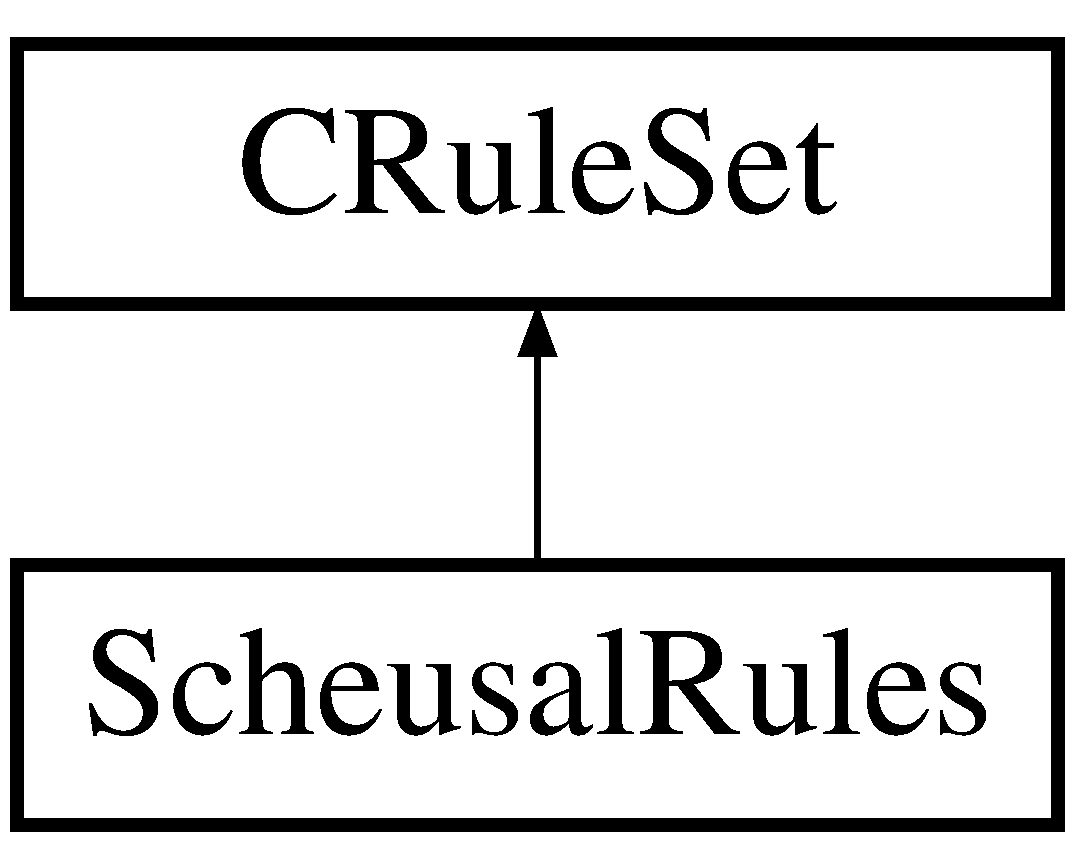
\includegraphics[height=2.000000cm]{class_scheusal_rules}
\end{center}
\end{figure}
\subsection*{Public Member Functions}
\begin{DoxyCompactItemize}
\item 
\mbox{\Hypertarget{class_scheusal_rules_a69f27ad6633b1e52496b9a6ffffad48d}\label{class_scheusal_rules_a69f27ad6633b1e52496b9a6ffffad48d}} 
{\bfseries Scheusal\+Rules} (\hyperlink{classmfg_1_1_engine}{mfg\+::\+Engine} $\ast$ge)
\item 
\mbox{\Hypertarget{class_scheusal_rules_a1d73e8287bb6c822cd6e6285522dd1bf}\label{class_scheusal_rules_a1d73e8287bb6c822cd6e6285522dd1bf}} 
virtual void {\bfseries apply} (\hyperlink{class_actor}{Actor} $\ast$)
\end{DoxyCompactItemize}
\subsection*{Additional Inherited Members}


\subsection{Detailed Description}
The \hyperlink{class_scheusal_rules}{Scheusal\+Rules} class -\/ Rule set for a Scheusal (Zombie) 

The documentation for this class was generated from the following files\+:\begin{DoxyCompactItemize}
\item 
scheusalrules.\+h\item 
scheusalrules.\+cpp\end{DoxyCompactItemize}

\hypertarget{class_sequential_g_u_i_d}{}\section{Sequential\+G\+U\+ID Class Reference}
\label{class_sequential_g_u_i_d}\index{Sequential\+G\+U\+ID@{Sequential\+G\+U\+ID}}


The \hyperlink{class_sequential_g_u_i_d}{Sequential\+G\+U\+ID} class -\/ define a class for creating a Sequential G\+U\+ID.  




{\ttfamily \#include $<$sequentialguid.\+h$>$}

Inheritance diagram for Sequential\+G\+U\+ID\+:\begin{figure}[H]
\begin{center}
\leavevmode
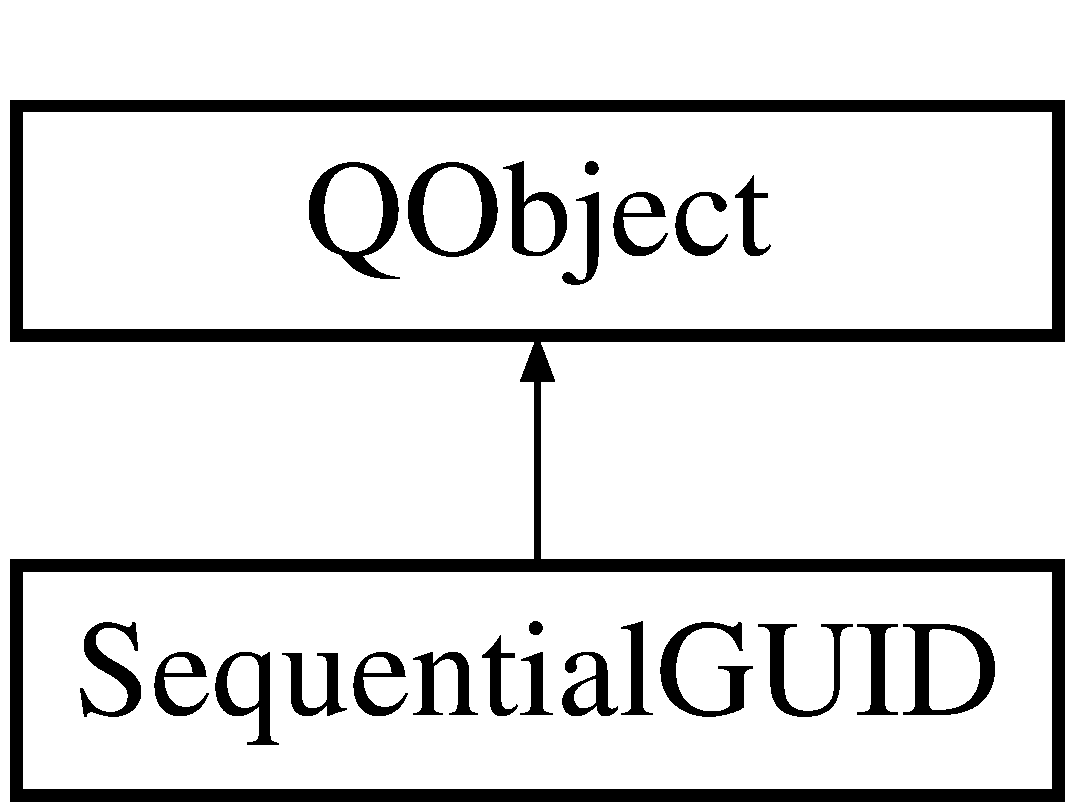
\includegraphics[height=2.000000cm]{class_sequential_g_u_i_d}
\end{center}
\end{figure}
\subsection*{Public Types}
\begin{DoxyCompactItemize}
\item 
\mbox{\Hypertarget{class_sequential_g_u_i_d_a085c09b21b940489a82002cc044ed6ea}\label{class_sequential_g_u_i_d_a085c09b21b940489a82002cc044ed6ea}} 
enum {\bfseries Sequential\+G\+U\+I\+D\+Type} \{ {\bfseries Sequential\+As\+String} = 0, 
{\bfseries Sequential\+As\+Binary} = 1, 
{\bfseries Sequential\+At\+End} = 2
 \}
\end{DoxyCompactItemize}
\subsection*{Public Member Functions}
\begin{DoxyCompactItemize}
\item 
\mbox{\Hypertarget{class_sequential_g_u_i_d_a0e87930b667cd86c011099c287961421}\label{class_sequential_g_u_i_d_a0e87930b667cd86c011099c287961421}} 
{\bfseries Sequential\+G\+U\+ID} (Q\+Object $\ast$parent=0)
\end{DoxyCompactItemize}
\subsection*{Static Public Member Functions}
\begin{DoxyCompactItemize}
\item 
\mbox{\Hypertarget{class_sequential_g_u_i_d_a25eea64f60dd43c7c21539f7b47a82e2}\label{class_sequential_g_u_i_d_a25eea64f60dd43c7c21539f7b47a82e2}} 
static Q\+Uuid {\bfseries Get\+Sequential\+G\+U\+ID} (Sequential\+G\+U\+I\+D\+Type guid\+\_\+type)
\end{DoxyCompactItemize}
\subsection*{Static Private Member Functions}
\begin{DoxyCompactItemize}
\item 
\mbox{\Hypertarget{class_sequential_g_u_i_d_ac9cd3532db46758fd4bbe990857cf9d7}\label{class_sequential_g_u_i_d_ac9cd3532db46758fd4bbe990857cf9d7}} 
static void {\bfseries Init\+Rand} ()
\item 
\mbox{\Hypertarget{class_sequential_g_u_i_d_ad1613a94f41f66eff11b36f0110e824a}\label{class_sequential_g_u_i_d_ad1613a94f41f66eff11b36f0110e824a}} 
static int {\bfseries rand\+Int} (int low, int high)
\end{DoxyCompactItemize}
\subsection*{Static Private Attributes}
\begin{DoxyCompactItemize}
\item 
\mbox{\Hypertarget{class_sequential_g_u_i_d_a9744b485ad5921199796cc014b7cb831}\label{class_sequential_g_u_i_d_a9744b485ad5921199796cc014b7cb831}} 
static bool {\bfseries rand\+\_\+init} = false
\end{DoxyCompactItemize}


\subsection{Detailed Description}
The \hyperlink{class_sequential_g_u_i_d}{Sequential\+G\+U\+ID} class -\/ define a class for creating a Sequential G\+U\+ID. 

The documentation for this class was generated from the following files\+:\begin{DoxyCompactItemize}
\item 
sequentialguid.\+h\item 
sequentialguid.\+cpp\end{DoxyCompactItemize}

\hypertarget{class_sprite}{}\section{Sprite Class Reference}
\label{class_sprite}\index{Sprite@{Sprite}}


The \hyperlink{class_sprite}{Sprite} class -\/ defines a \hyperlink{class_sprite}{Sprite}.  




{\ttfamily \#include $<$sprite.\+h$>$}

Inheritance diagram for Sprite\+:\begin{figure}[H]
\begin{center}
\leavevmode
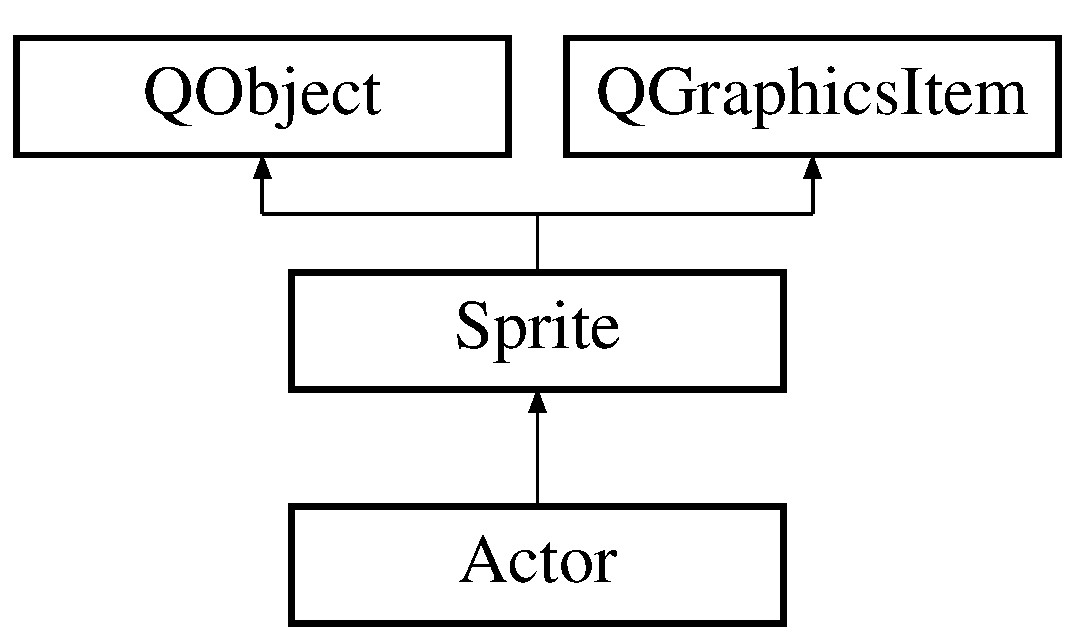
\includegraphics[height=3.000000cm]{class_sprite}
\end{center}
\end{figure}
\subsection*{Public Slots}
\begin{DoxyCompactItemize}
\item 
\mbox{\Hypertarget{class_sprite_ab76c12803dcd1f7a44c4acbbec91380d}\label{class_sprite_ab76c12803dcd1f7a44c4acbbec91380d}} 
virtual void {\bfseries mouse\+Press\+Event} (Q\+Graphics\+Scene\+Mouse\+Event $\ast$event) override
\item 
\mbox{\Hypertarget{class_sprite_a8935559355be47d8ba7e7eb175aecdb5}\label{class_sprite_a8935559355be47d8ba7e7eb175aecdb5}} 
virtual void {\bfseries animate} ()
\end{DoxyCompactItemize}
\subsection*{Signals}
\begin{DoxyCompactItemize}
\item 
\mbox{\Hypertarget{class_sprite_aa3e462d06474d09e40c5a793794622f8}\label{class_sprite_aa3e462d06474d09e40c5a793794622f8}} 
void {\bfseries sprite\+Click} (Q\+Graphics\+Scene\+Mouse\+Event $\ast$, \hyperlink{class_sprite}{Sprite} $\ast$)
\item 
\mbox{\Hypertarget{class_sprite_a48ccbc5c26c6071cb179a243247c1250}\label{class_sprite_a48ccbc5c26c6071cb179a243247c1250}} 
void {\bfseries sprite\+Move} (\hyperlink{class_sprite}{Sprite} $\ast$)
\item 
\mbox{\Hypertarget{class_sprite_aac4537dfb67bc626f96e78fa09295f9b}\label{class_sprite_aac4537dfb67bc626f96e78fa09295f9b}} 
void {\bfseries action\+Changed} (\hyperlink{class_sprite}{Sprite} $\ast$)
\item 
\mbox{\Hypertarget{class_sprite_a310fe32fd00d8f7a61f5a7a0dfb83c9b}\label{class_sprite_a310fe32fd00d8f7a61f5a7a0dfb83c9b}} 
void {\bfseries sprite\+Collision} (\hyperlink{class_sprite}{Sprite} $\ast$, Sprite\+List $\ast$)
\item 
\mbox{\Hypertarget{class_sprite_a54745b981741c82b59e65824752ba12e}\label{class_sprite_a54745b981741c82b59e65824752ba12e}} 
void {\bfseries sprite\+Painting} (\hyperlink{class_sprite}{Sprite} $\ast$, Q\+Painter $\ast$painter, const Q\+Style\+Option\+Graphics\+Item $\ast$option, Q\+Widget $\ast$widget)
\end{DoxyCompactItemize}
\subsection*{Public Member Functions}
\begin{DoxyCompactItemize}
\item 
\mbox{\Hypertarget{class_sprite_a0f5230614f211b04056a376b83ecd9e5}\label{class_sprite_a0f5230614f211b04056a376b83ecd9e5}} 
{\bfseries Sprite} (const Q\+String \&name, \hyperlink{classmfg_1_1_engine}{mfg\+::\+Engine} $\ast$engine, bool moving, Q\+Object $\ast$parent=0)
\item 
\mbox{\Hypertarget{class_sprite_a8cc9c3ebeab9f25834f1f8c171880e0e}\label{class_sprite_a8cc9c3ebeab9f25834f1f8c171880e0e}} 
Sprite\+\_\+\+Direction {\bfseries direction} ()
\item 
\mbox{\Hypertarget{class_sprite_a69ced4a3db80daf660bdbc2e9aced096}\label{class_sprite_a69ced4a3db80daf660bdbc2e9aced096}} 
void {\bfseries direction} (Sprite\+\_\+\+Direction d)
\item 
\mbox{\Hypertarget{class_sprite_a9b0acb015439554398b064411d3e0ab9}\label{class_sprite_a9b0acb015439554398b064411d3e0ab9}} 
virtual Q\+String {\bfseries name} () const
\item 
\mbox{\Hypertarget{class_sprite_af14553ba4a7bb1234f336f42e5162915}\label{class_sprite_af14553ba4a7bb1234f336f42e5162915}} 
void {\bfseries name} (const Q\+String \&name)
\item 
\mbox{\Hypertarget{class_sprite_a67ca36798b90d7365e52555dbc0d2c2e}\label{class_sprite_a67ca36798b90d7365e52555dbc0d2c2e}} 
bool {\bfseries is\+Colliding} ()
\item 
\mbox{\Hypertarget{class_sprite_a1b0178ef50baf6b4c14f94d3c68ab595}\label{class_sprite_a1b0178ef50baf6b4c14f94d3c68ab595}} 
void {\bfseries collision\+State} (Collision\+\_\+\+State)
\item 
\mbox{\Hypertarget{class_sprite_a1a702eca5ba1fc379918dffdfb90e7c2}\label{class_sprite_a1a702eca5ba1fc379918dffdfb90e7c2}} 
Q\+Brush {\bfseries get\+Collision\+Brush} ()
\item 
\mbox{\Hypertarget{class_sprite_a49e10268cfc2bec206820d224c892e2c}\label{class_sprite_a49e10268cfc2bec206820d224c892e2c}} 
Collision\+\_\+\+State {\bfseries collision\+State} ()
\item 
\mbox{\Hypertarget{class_sprite_a683492949abb6ef283debc24a97b3535}\label{class_sprite_a683492949abb6ef283debc24a97b3535}} 
Sprite\+List {\bfseries colliding\+List} ()
\item 
\mbox{\Hypertarget{class_sprite_a67a8273fc7db9ed534cca3957d1a0598}\label{class_sprite_a67a8273fc7db9ed534cca3957d1a0598}} 
bool {\bfseries is\+Sprite} (const Q\+Graphics\+Item $\ast$item)
\item 
\mbox{\Hypertarget{class_sprite_a289c85c632dfcafe8cc378c649d8375c}\label{class_sprite_a289c85c632dfcafe8cc378c649d8375c}} 
\hyperlink{classmfg_1_1_engine}{mfg\+::\+Engine} $\ast$ {\bfseries gameengine} ()
\item 
\mbox{\Hypertarget{class_sprite_abe1915f40313eaca777665dc041440ab}\label{class_sprite_abe1915f40313eaca777665dc041440ab}} 
\hyperlink{class_asset_manager}{Asset\+Manager} $\ast$ {\bfseries assetmanager} ()
\item 
\mbox{\Hypertarget{class_sprite_ad690815ac85d948a52a1136596037c67}\label{class_sprite_ad690815ac85d948a52a1136596037c67}} 
Sprite\+Frames\+Map {\bfseries sprite\+Frames} ()
\item 
\mbox{\Hypertarget{class_sprite_a2c6faefb1b08c2a87d6b0562f3577e6f}\label{class_sprite_a2c6faefb1b08c2a87d6b0562f3577e6f}} 
Sprite\+Frames\+Map {\bfseries add\+Sprite\+Frame\+Coordinates} (const Q\+String \&name, Coordinates coord)
\item 
\mbox{\Hypertarget{class_sprite_a6dccaa6d6fca24fc01a7a48542bc3fa2}\label{class_sprite_a6dccaa6d6fca24fc01a7a48542bc3fa2}} 
int {\bfseries sprite\+Size} ()
\item 
\mbox{\Hypertarget{class_sprite_a2891012b8636c18d38b244bc54d31c03}\label{class_sprite_a2891012b8636c18d38b244bc54d31c03}} 
Q\+Uuid {\bfseries guid} () const
\item 
\mbox{\Hypertarget{class_sprite_a55b47ce9303d5b2ac9b4a2e48f8baacc}\label{class_sprite_a55b47ce9303d5b2ac9b4a2e48f8baacc}} 
void {\bfseries guid} (const Q\+Uuid \&guid)
\item 
\mbox{\Hypertarget{class_sprite_a3fb65e4969ae7c92278513e187d4d2db}\label{class_sprite_a3fb65e4969ae7c92278513e187d4d2db}} 
int {\bfseries current\+\_\+frame} () const
\item 
\mbox{\Hypertarget{class_sprite_acad9e57881565704cce66f6a9f25b553}\label{class_sprite_acad9e57881565704cce66f6a9f25b553}} 
void {\bfseries current\+\_\+frame} (int current\+\_\+frame)
\item 
\mbox{\Hypertarget{class_sprite_aa5e9083132f0431a76e64eaad2c37d0b}\label{class_sprite_aa5e9083132f0431a76e64eaad2c37d0b}} 
int {\bfseries advance\+\_\+frame} (int)
\item 
\mbox{\Hypertarget{class_sprite_af1e07744e99034cbcaea64d0cb6d7de3}\label{class_sprite_af1e07744e99034cbcaea64d0cb6d7de3}} 
float {\bfseries advance\+\_\+distance} () const
\item 
\mbox{\Hypertarget{class_sprite_a91d7d4c46a38c58fa1ef05c4132e5fcf}\label{class_sprite_a91d7d4c46a38c58fa1ef05c4132e5fcf}} 
void {\bfseries advance\+\_\+distance} (float advance\+\_\+distance)
\item 
\mbox{\Hypertarget{class_sprite_a4482fc0a1581aaf91c97175a79be319a}\label{class_sprite_a4482fc0a1581aaf91c97175a79be319a}} 
int {\bfseries sprite\+\_\+image\+\_\+top} () const
\item 
\mbox{\Hypertarget{class_sprite_a7f5f82520ed2901d7fc89f01d981a49f}\label{class_sprite_a7f5f82520ed2901d7fc89f01d981a49f}} 
void {\bfseries sprite\+\_\+image\+\_\+top} (int sprite\+\_\+image\+\_\+top)
\item 
\mbox{\Hypertarget{class_sprite_a9a139be20b5b5a5237c9a81b36f625f8}\label{class_sprite_a9a139be20b5b5a5237c9a81b36f625f8}} 
int {\bfseries sprite\+\_\+image\+\_\+left} () const
\item 
\mbox{\Hypertarget{class_sprite_a92d9872ab695420bc81ede2a9425aeea}\label{class_sprite_a92d9872ab695420bc81ede2a9425aeea}} 
void {\bfseries sprite\+\_\+image\+\_\+left} (int sprite\+\_\+image\+\_\+left)
\item 
\mbox{\Hypertarget{class_sprite_af9153229a8327b4d247ef16448c1cb35}\label{class_sprite_af9153229a8327b4d247ef16448c1cb35}} 
bool {\bfseries animating} () const
\item 
\mbox{\Hypertarget{class_sprite_a1a3df748d6a3469d1b79cde39adb8ebc}\label{class_sprite_a1a3df748d6a3469d1b79cde39adb8ebc}} 
void {\bfseries animating} (bool animating)
\item 
\mbox{\Hypertarget{class_sprite_a55f3a0b845fc21ff9f0774613124b1e6}\label{class_sprite_a55f3a0b845fc21ff9f0774613124b1e6}} 
void {\bfseries update\+\_\+sprite} ()
\item 
\mbox{\Hypertarget{class_sprite_acdba2a71fac359258d583bcdc2648cdd}\label{class_sprite_acdba2a71fac359258d583bcdc2648cdd}} 
int {\bfseries sprite\+\_\+width} () const
\item 
\mbox{\Hypertarget{class_sprite_a767f74c47c154fccb06d815a1ba33561}\label{class_sprite_a767f74c47c154fccb06d815a1ba33561}} 
int {\bfseries sprite\+\_\+height} () const
\item 
\mbox{\Hypertarget{class_sprite_acebb5f6a962000aae733d919e2a6392d}\label{class_sprite_acebb5f6a962000aae733d919e2a6392d}} 
bool {\bfseries stationary} () const
\item 
\mbox{\Hypertarget{class_sprite_ab05f29a527cec4d079c1ed74c8980d3c}\label{class_sprite_ab05f29a527cec4d079c1ed74c8980d3c}} 
int {\bfseries animation\+\_\+cells} () const
\item 
\mbox{\Hypertarget{class_sprite_a54ab5cb9dc016b0fc26eb465b3b792c3}\label{class_sprite_a54ab5cb9dc016b0fc26eb465b3b792c3}} 
void {\bfseries animation\+\_\+cells} (int animation\+\_\+cells)
\end{DoxyCompactItemize}
\subsection*{Protected Member Functions}
\begin{DoxyCompactItemize}
\item 
\mbox{\Hypertarget{class_sprite_a73230a5034b8d9091a3e31fbdd3b0d46}\label{class_sprite_a73230a5034b8d9091a3e31fbdd3b0d46}} 
virtual void {\bfseries paint} (Q\+Painter $\ast$painter, const Q\+Style\+Option\+Graphics\+Item $\ast$option, Q\+Widget $\ast$widget) override
\item 
\mbox{\Hypertarget{class_sprite_a48de16f5c8661ef4700ab7a411aebded}\label{class_sprite_a48de16f5c8661ef4700ab7a411aebded}} 
virtual void \hyperlink{class_sprite_a48de16f5c8661ef4700ab7a411aebded}{advance} (int step) Q\+\_\+\+D\+E\+C\+L\+\_\+\+O\+V\+E\+R\+R\+I\+DE
\begin{DoxyCompactList}\small\item\em Sprite\+::next\+Frame Will set the frame as well as the position of the sprite in the scene. \end{DoxyCompactList}\item 
\mbox{\Hypertarget{class_sprite_a0af8ed7bce1d1dde0a2c01f9461d4b4f}\label{class_sprite_a0af8ed7bce1d1dde0a2c01f9461d4b4f}} 
void {\bfseries build\+Coordinates} ()
\item 
\mbox{\Hypertarget{class_sprite_aefcdf13598b88f1ad0a4bfd797815b3b}\label{class_sprite_aefcdf13598b88f1ad0a4bfd797815b3b}} 
void {\bfseries check\+If\+Out\+Of\+Bounds} ()
\item 
\mbox{\Hypertarget{class_sprite_aaa1b06057132ee51960b783635cfec44}\label{class_sprite_aaa1b06057132ee51960b783635cfec44}} 
void {\bfseries check\+Collision} ()
\item 
\mbox{\Hypertarget{class_sprite_a642055fcd741b2c205a9a1359ce0b30f}\label{class_sprite_a642055fcd741b2c205a9a1359ce0b30f}} 
Q\+RectF {\bfseries bounding\+Rect} () const override
\end{DoxyCompactItemize}
\subsection*{Protected Attributes}
\begin{DoxyCompactItemize}
\item 
\mbox{\Hypertarget{class_sprite_a7255ed65d71ab4a5dac9ad60d3df19b9}\label{class_sprite_a7255ed65d71ab4a5dac9ad60d3df19b9}} 
Q\+String {\bfseries m\+\_\+sprite\+\_\+name}
\item 
\mbox{\Hypertarget{class_sprite_ad9cb2135f3b3d7ca71b3ebdef7b46c56}\label{class_sprite_ad9cb2135f3b3d7ca71b3ebdef7b46c56}} 
bool {\bfseries m\+\_\+animated}
\item 
\mbox{\Hypertarget{class_sprite_a23d8bfff2dcbe87094e8eb625c3497ec}\label{class_sprite_a23d8bfff2dcbe87094e8eb625c3497ec}} 
bool {\bfseries m\+\_\+stationary}
\item 
\mbox{\Hypertarget{class_sprite_a38a7b0f7ae13e13468307dabd7bc0b1c}\label{class_sprite_a38a7b0f7ae13e13468307dabd7bc0b1c}} 
bool {\bfseries m\+\_\+collision}
\item 
\mbox{\Hypertarget{class_sprite_a5dd4426e4ffce9fd4b5038205d8ca4e4}\label{class_sprite_a5dd4426e4ffce9fd4b5038205d8ca4e4}} 
Collision\+\_\+\+State {\bfseries m\+\_\+collision\+\_\+state}
\item 
\mbox{\Hypertarget{class_sprite_a491078bf7e9b7fce4f879cec717730a3}\label{class_sprite_a491078bf7e9b7fce4f879cec717730a3}} 
int {\bfseries m\+\_\+sprite\+\_\+width}
\item 
\mbox{\Hypertarget{class_sprite_a24e431a38ed3550f6159c38eedf3b040}\label{class_sprite_a24e431a38ed3550f6159c38eedf3b040}} 
int {\bfseries m\+\_\+sprite\+\_\+height}
\item 
\mbox{\Hypertarget{class_sprite_a02e24d304f28386e583db76033c90807}\label{class_sprite_a02e24d304f28386e583db76033c90807}} 
int {\bfseries m\+\_\+sprite\+\_\+speed}
\item 
\mbox{\Hypertarget{class_sprite_a623b2ec261659d243b10b4cc2e4207bf}\label{class_sprite_a623b2ec261659d243b10b4cc2e4207bf}} 
Q\+Pixmap $\ast$ {\bfseries m\+\_\+pixmap}
\item 
\mbox{\Hypertarget{class_sprite_abfb8dabc8cd79ae3101d50d87e8a356c}\label{class_sprite_abfb8dabc8cd79ae3101d50d87e8a356c}} 
float {\bfseries m\+\_\+advance\+\_\+distance}
\item 
\mbox{\Hypertarget{class_sprite_aecb4f20e0c6ac5c0e4ca13ebd2ad019d}\label{class_sprite_aecb4f20e0c6ac5c0e4ca13ebd2ad019d}} 
int {\bfseries m\+\_\+left\+\_\+adjust}
\item 
\mbox{\Hypertarget{class_sprite_ac12b46153b557acad91b0763377a8747}\label{class_sprite_ac12b46153b557acad91b0763377a8747}} 
int {\bfseries m\+\_\+top\+\_\+adjust}
\item 
\mbox{\Hypertarget{class_sprite_aa53eecf1c0313b0530aa8e87364e5483}\label{class_sprite_aa53eecf1c0313b0530aa8e87364e5483}} 
int {\bfseries m\+\_\+right\+\_\+adjust}
\item 
\mbox{\Hypertarget{class_sprite_a5e9335a279146b9d6a39732286f66442}\label{class_sprite_a5e9335a279146b9d6a39732286f66442}} 
int {\bfseries m\+\_\+bottom\+\_\+adjust}
\item 
\mbox{\Hypertarget{class_sprite_a0cbe2eea79406aa5eab79f3271f5c901}\label{class_sprite_a0cbe2eea79406aa5eab79f3271f5c901}} 
int {\bfseries m\+\_\+sprite\+\_\+image\+\_\+top}
\item 
\mbox{\Hypertarget{class_sprite_a1bb7b306f6c0387a8f5650a4e45daddd}\label{class_sprite_a1bb7b306f6c0387a8f5650a4e45daddd}} 
int {\bfseries m\+\_\+sprite\+\_\+image\+\_\+left}
\item 
\mbox{\Hypertarget{class_sprite_a4a6bdd8069db054217442c6b8aead52a}\label{class_sprite_a4a6bdd8069db054217442c6b8aead52a}} 
int {\bfseries m\+\_\+start\+\_\+row}
\item 
\mbox{\Hypertarget{class_sprite_a2314213e4197f42f810e48f1243f8596}\label{class_sprite_a2314213e4197f42f810e48f1243f8596}} 
int {\bfseries m\+\_\+start\+\_\+col}
\item 
\mbox{\Hypertarget{class_sprite_ad644cf3253e4b3371e225726f8e9dacc}\label{class_sprite_ad644cf3253e4b3371e225726f8e9dacc}} 
int {\bfseries m\+\_\+sprite\+\_\+rows}
\item 
\mbox{\Hypertarget{class_sprite_a80844771769275623be3247941459e11}\label{class_sprite_a80844771769275623be3247941459e11}} 
int {\bfseries m\+\_\+sprite\+\_\+cols}
\item 
\mbox{\Hypertarget{class_sprite_ac88ed94b6860902cecb17951ce9875ff}\label{class_sprite_ac88ed94b6860902cecb17951ce9875ff}} 
int {\bfseries m\+\_\+animation\+\_\+cells}
\item 
\mbox{\Hypertarget{class_sprite_a2e9f094a7a7e6437e9577fb588060bab}\label{class_sprite_a2e9f094a7a7e6437e9577fb588060bab}} 
Sprite\+\_\+\+Direction {\bfseries m\+\_\+current\+\_\+direction}
\item 
\mbox{\Hypertarget{class_sprite_ac73ca0065a580f0ea4e9a326b978b4b1}\label{class_sprite_ac73ca0065a580f0ea4e9a326b978b4b1}} 
int {\bfseries m\+\_\+current\+\_\+frame}
\item 
\mbox{\Hypertarget{class_sprite_a021bef47963b5be8b19ba755015d8ac1}\label{class_sprite_a021bef47963b5be8b19ba755015d8ac1}} 
Sprite\+Frames\+Map {\bfseries m\+\_\+sprite\+\_\+frames}
\item 
\mbox{\Hypertarget{class_sprite_a4e0c8c16649b6f95e87c1af002f4375a}\label{class_sprite_a4e0c8c16649b6f95e87c1af002f4375a}} 
Sprite\+List {\bfseries m\+\_\+colliding\+\_\+list}
\item 
\mbox{\Hypertarget{class_sprite_af29e1d71cf77027699b3976598d6732c}\label{class_sprite_af29e1d71cf77027699b3976598d6732c}} 
\hyperlink{class_asset_manager}{Asset\+Manager} $\ast$ {\bfseries m\+\_\+asset\+\_\+manager}
\item 
\mbox{\Hypertarget{class_sprite_adad80bf689553b255a77881a8a0d21a7}\label{class_sprite_adad80bf689553b255a77881a8a0d21a7}} 
\hyperlink{classmfg_1_1_engine}{mfg\+::\+Engine} $\ast$ {\bfseries m\+\_\+game\+\_\+engine}
\item 
\mbox{\Hypertarget{class_sprite_ad19296749b5cd1f97e28163386d08f1e}\label{class_sprite_ad19296749b5cd1f97e28163386d08f1e}} 
Q\+Uuid {\bfseries m\+\_\+guid}
\end{DoxyCompactItemize}


\subsection{Detailed Description}
The \hyperlink{class_sprite}{Sprite} class -\/ defines a \hyperlink{class_sprite}{Sprite}. 

The documentation for this class was generated from the following files\+:\begin{DoxyCompactItemize}
\item 
sprite.\+h\item 
sprite.\+cpp\end{DoxyCompactItemize}

\hypertarget{structmfg_1_1_stats}{}\section{mfg\+:\+:Stats Struct Reference}
\label{structmfg_1_1_stats}\index{mfg\+::\+Stats@{mfg\+::\+Stats}}


The \hyperlink{structmfg_1_1_stats}{Stats} struct -\/ defines the stats for a character.  




{\ttfamily \#include $<$gameengine.\+h$>$}

\subsection*{Public Attributes}
\begin{DoxyCompactItemize}
\item 
\mbox{\Hypertarget{structmfg_1_1_stats_a1170cdacbc82425eb2801a1220582da3}\label{structmfg_1_1_stats_a1170cdacbc82425eb2801a1220582da3}} 
int {\bfseries health}
\item 
\mbox{\Hypertarget{structmfg_1_1_stats_aa4a344305e9e1eb4e7ac617c538c3bf1}\label{structmfg_1_1_stats_aa4a344305e9e1eb4e7ac617c538c3bf1}} 
int {\bfseries stamina}
\item 
\mbox{\Hypertarget{structmfg_1_1_stats_adc3325405ac0550c7017eb2a369d7c86}\label{structmfg_1_1_stats_adc3325405ac0550c7017eb2a369d7c86}} 
int {\bfseries wealth}
\item 
\mbox{\Hypertarget{structmfg_1_1_stats_adf21a6f756e7cbabb974d5395ada1b89}\label{structmfg_1_1_stats_adf21a6f756e7cbabb974d5395ada1b89}} 
int {\bfseries manna}
\item 
\mbox{\Hypertarget{structmfg_1_1_stats_a78e5181b5830ceb7c4c71b32b59578c8}\label{structmfg_1_1_stats_a78e5181b5830ceb7c4c71b32b59578c8}} 
int {\bfseries life}
\end{DoxyCompactItemize}


\subsection{Detailed Description}
The \hyperlink{structmfg_1_1_stats}{Stats} struct -\/ defines the stats for a character. 

The documentation for this struct was generated from the following file\+:\begin{DoxyCompactItemize}
\item 
gameengine.\+h\end{DoxyCompactItemize}

\hypertarget{class_utilities}{}\section{Utilities Class Reference}
\label{class_utilities}\index{Utilities@{Utilities}}


The \hyperlink{class_utilities}{Utilities} class -\/ defines a \hyperlink{class_utilities}{Utilities} class for functions required, mostly static functions.  




{\ttfamily \#include $<$utilities.\+h$>$}

\subsection*{Static Public Member Functions}
\begin{DoxyCompactItemize}
\item 
\mbox{\Hypertarget{class_utilities_ab8d1ca3ddf49e268e7bc2669da100369}\label{class_utilities_ab8d1ca3ddf49e268e7bc2669da100369}} 
static int {\bfseries rand\+Int} (int low, int high)
\end{DoxyCompactItemize}


\subsection{Detailed Description}
The \hyperlink{class_utilities}{Utilities} class -\/ defines a \hyperlink{class_utilities}{Utilities} class for functions required, mostly static functions. 

The documentation for this class was generated from the following files\+:\begin{DoxyCompactItemize}
\item 
utilities.\+h\item 
utilities.\+cpp\end{DoxyCompactItemize}

\hypertarget{class_villager_rules}{}\section{Villager\+Rules Class Reference}
\label{class_villager_rules}\index{Villager\+Rules@{Villager\+Rules}}
Inheritance diagram for Villager\+Rules\+:\begin{figure}[H]
\begin{center}
\leavevmode
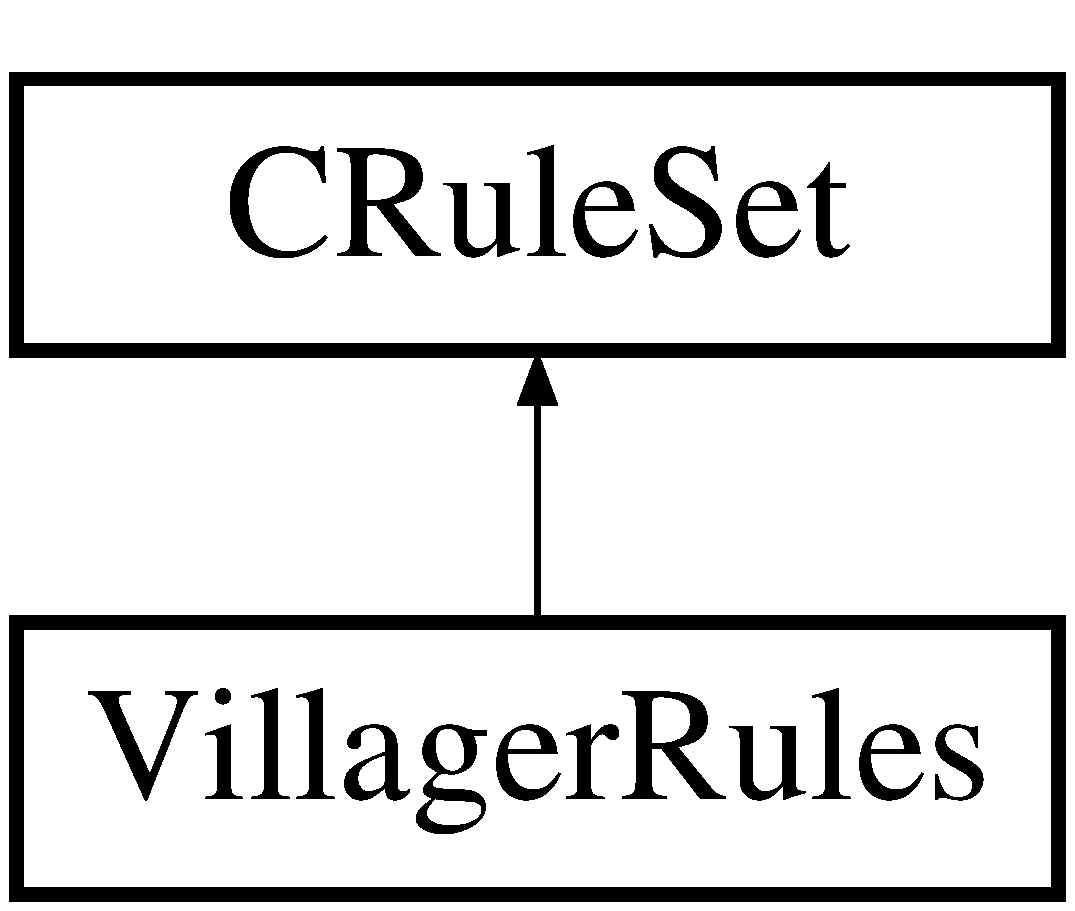
\includegraphics[height=2.000000cm]{class_villager_rules}
\end{center}
\end{figure}
\subsection*{Public Member Functions}
\begin{DoxyCompactItemize}
\item 
\mbox{\Hypertarget{class_villager_rules_a7c23dd17126f9d1c1e1b9ada7f965bff}\label{class_villager_rules_a7c23dd17126f9d1c1e1b9ada7f965bff}} 
{\bfseries Villager\+Rules} (\hyperlink{classmfg_1_1_engine}{mfg\+::\+Engine} $\ast$ge)
\item 
\mbox{\Hypertarget{class_villager_rules_ac78c4a1461517c37bd860033a82b75d3}\label{class_villager_rules_ac78c4a1461517c37bd860033a82b75d3}} 
virtual void {\bfseries apply} (\hyperlink{class_actor}{Actor} $\ast$)
\end{DoxyCompactItemize}
\subsection*{Additional Inherited Members}


The documentation for this class was generated from the following files\+:\begin{DoxyCompactItemize}
\item 
villagerrules.\+h\item 
villagerrules.\+cpp\end{DoxyCompactItemize}

%--- End generated contents ---

% Index
\backmatter
\newpage
\phantomsection
\clearemptydoublepage
\addcontentsline{toc}{chapter}{Index}
\printindex

\end{document}
